% !TEX root = ../OT4ML.tex

%%%%%%%%%%%%%%%%%%%%%%%%%%%%%%%%%%%%%%%%%%%%%%%%%%%%%%%%%%%%%%%%%%%%%%%%%%%
%%%%%%%%%%%%%%%%%%%%%%%%%%%%%%%%%%%%%%%%%%%%%%%%%%%%%%%%%%%%%%%%%%%%%%%%%%%
%%%%%%%%%%%%%%%%%%%%%%%%%%%%%%%%%%%%%%%%%%%%%%%%%%%%%%%%%%%%%%%%%%%%%%%%%%%
\chapter{Entropic Regularization: Convergence}
\index{entropic!regularization}% strictindex
\index{Sinkhorn!convergence}% strictindex
\label{sec-sinkhorn-advanced}
\label{sec-entropic-convergence}
\label{sec-convergence-dual}

This chapter focuses on algorithmic convergence for entropic optimal transport: the marginals and the temperature are fixed, and one asks how Sinkhorn iterates, soft transforms and related monotone scaling procedures approach their regularized fixed point. Statistical convergence is a separate question, because the empirical marginals then change with the sample size; this is the topic of Chapter~\ref{sec-statistical-ot}.
\index{algorithmic convergence}% strictindex
\index{Sinkhorn!fixed point}% strictindex
\index{matrix!scaling}% strictindex
\index{soft!transform}% strictindex

The chapter revisits Sinkhorn convergence through several complementary lenses. Bregman projections explain the alternating-projection geometry, while Fortet's order argument gives qualitative fixed-point convergence. Robust Bregman estimates then give a non-asymptotic $O(1/\ell)$ dual-gap bound, and Hilbert's metric gives a clean global linear contraction when the kernel is uniformly positive. A local spectral analysis sharpens this factor and motivates over-relaxation and variable projection. The last sections discuss Gaussian closed forms and continuous \(\varepsilon\)-Sinkhorn flows as model cases where the fixed-point structure becomes explicit.
\index{Sinkhorn!convergence}% strictindex
\index{Bregman!projection}% strictindex
\index{dual!gap}% strictindex

%%%%%%%%%%%%%%%%%%%%%%%%%%%%%%%%%%%%%%%%%%%%%%%%%%%%%%%%%%%%%%%%%%%%%%%%%%%
\section{Sinkhorn Convergence: Bregman Point of View}
\label{sec-convergence-init}

This section explains Sinkhorn as alternating Bregman projections. The main message is geometric: each row or column rescaling is the KL projection onto one affine marginal constraint, so convergence follows from the Pythagorean identity for Bregman divergences.
\index{Kullback-Leibler@Kullback--Leibler!projection}% strictindex
\index{marginal!constraint}% strictindex
\index{affine!marginal constraint}% strictindex
\index{Pythagorean identity}% strictindex
\index{Bregman!divergence}% strictindex
\index{Bregman!projection}% strictindex

For simplicity, this section is written for discrete measures, but the same ideas carry over to general measures. The robust-rate section later revisits the alternating-projection mechanism through convex duality, with constants expressed through the oscillation of the potentials and of the cost range.

\paragraph{Alternating $\KL$ projections.}
\index{alternating!projection}% strictindex

The projection viewpoint explains Sinkhorn as repeated enforcement of one marginal constraint at a time. It is not specific to entropy, although the KL case is the one where the projections reduce to elementary row and column scalings.
\index{scaling!row}% strictindex
\index{scaling!column}% strictindex
\index{marginal!constraint}% strictindex

The following matrix construction is the finite-dimensional counterpart of the measure-valued Definition~\ref{def-measure-bregman-divergence}.

\begin{defn}[Bregman divergence]\label{def-bregman-divergence}
\index{Bregman!divergence}% strictindex
	Let $\Omega\subset\RR^{n\times m}$ be convex with nonempty interior, and let $\Phi:\RR^{n\times m}\to\RR\cup\{+\infty\}$ be a proper lower-semicontinuous Legendre function with $\operatorname{dom}(\Phi)=\Omega$. Thus $\Phi=+\infty$ outside $\Omega$, while $\Phi$ is differentiable and strictly convex on $\operatorname{int}(\Omega)$. For $\P,\Q\in\operatorname{int}(\Omega)$, the Bregman divergence generated by $\Phi$ is
\index{convex!function}% strictindex
	\index{Legendre function}% strictindex
	\[
		B_\Phi(\P|\Q)\eqdef \Phi(\P)-\Phi(\Q)-\dotp{\nabla\Phi(\Q)}{\P-\Q}.
	\]
\end{defn}

For the quadratic generator $\Phi(\P)=\frac12\norm{\P}_{\mathrm F}^2$ on $\RR^{n\times m}$, one recovers half the squared Euclidean distance, $B_\Phi(\P|\Q)=\frac12\norm{\P-\Q}_{\mathrm F}^2$. For the negative entropy $\Phi(\P)=\sum_{i,j}\P_{i,j}\log \P_{i,j}$ on the nonnegative orthant, extended by $+\infty$ outside it, one obtains $B_\Phi(\P|\Q)=\KLD(\P|\Q)$. For $\P\geq0$ and $\Q>0$, this identity is understood through the lower-semicontinuous extension, with $0\log0=0$.
\index{Frobenius norm}% strictindex
\index{negative Shannon entropy}% strictindex

The corresponding projection is the basic operation in alternating Bregman methods.
\begin{defn}[Bregman projection]\label{def-bregman-projection}
For a nonempty convex set $\Cc$, define
\[
	\Proj_{\Cc}^{B_\Phi}(\Q)
	\eqdef
	\argmin_{\P\in\Cc} B_\Phi(\P|\Q),
\]
which is set-valued if the minimizer is not unique.
\end{defn}

Bregman divergences are useful because their geometry can encode constraints. A Legendre-type generator $\Phi$ blows up, or has an infinite derivative, at the boundary of its domain. For negative entropy, positivity is therefore built into the divergence, so one projects onto affine marginal constraints without separately handling non-negativity.
\index{affine!marginal constraint}% strictindex
\index{marginal!constraint}% strictindex
\index{Bregman!divergence}% strictindex

\paragraph{Linear tilts and Gibbs references.}
\index{linear!tilt}% strictindex
\index{Gibbs!reference}% strictindex

The next proposition explains why adding a linear cost to a Bregman penalty merely shifts the reference point in dual coordinates. The usual Gibbs--KL reformulation is the entropy specialization.

\begin{prop}[Linear tilts of Bregman penalties]\label{prop-bregman-linear-tilt}
\index{Bregman!penalty}% strictindex
	Let $\Phi$ be differentiable and strictly convex, and let $B_\Phi$ be its Bregman divergence. Fix a reference point $\Q$ in the interior of the domain. Assume that there exists $\Q^\C$ such that
\index{Bregman!divergence}% strictindex
	\[
		\nabla\Phi(\Q^\C)=\nabla\Phi(\Q)-\C/\epsilon.
	\]
	Then, for all $\P$ in the domain,
	\[
		\dotp{\P}{\C}+\epsilon B_\Phi(\P|\Q)
		=
		\epsilon B_\Phi(\P|\Q^\C)+\text{\upshape cst},
	\]
	where the constant does not depend on $\P$.
\end{prop}
\begin{proof}
	Subtract the two Bregman divergences:
\index{Bregman!divergence}% strictindex
	\[
		B_\Phi(\P|\Q^\C)-B_\Phi(\P|\Q)
		=
		\dotp{\nabla\Phi(\Q)-\nabla\Phi(\Q^\C)}{\P}
		+\text{cst}.
	\]
	Using $\nabla\Phi(\Q)-\nabla\Phi(\Q^\C)=\C/\epsilon$ and multiplying by $\epsilon$ gives the claim.
\end{proof}

For the negative entropy $\Phi(\P)=\sum_{i,j}\P_{i,j}\log\P_{i,j}$, one has $B_\Phi=\KLD$. Taking $\Q=\a\otimes\b$ gives the tilted reference
\index{negative Shannon entropy}% strictindex
\[
	\K_{\a,\b}^\epsilon
	\eqdef
	(\a\otimes\b)\odot e^{-\C/\epsilon}.
\]
Thus
\[
	\dotp{\P}{\C}+\epsilon\KLD(\P|\a\otimes\b)
	=
	\epsilon\KLD(\P|\K_{\a,\b}^\epsilon)+\text{\upshape cst}.
\]
On the transport polytope, scaling $\K_{\a,\b}^\epsilon$ is equivalent to scaling the Gibbs kernel $\K=e^{-\C/\epsilon}$ because the factors $\a_i$ and $\b_j$ can be absorbed into the Sinkhorn scalings.
\index{Sinkhorn!scaling}% strictindex
\index{transportation polytope}% strictindex
\index{Gibbs!kernel}% strictindex

Thus the unique solution $\P_\epsilon$ of~\eqref{eq-regularized-discr} is the KL projection of the tilted Gibbs reference onto $\CouplingsD(\a,\b)$:
\index{Gibbs!reference}% strictindex
\index{Kullback-Leibler@Kullback--Leibler!projection}% strictindex
\eql{\label{eq-kl-proj}
	\P_\epsilon = \Proj_{\CouplingsD(\a,\b)}^\KLD(\K_{\a,\b}^\epsilon) \eqdef \uargmin{\P \in \CouplingsD(\a,\b)} \KLD(\P|\K_{\a,\b}^\epsilon).
}

\paragraph{Cyclic projection convergence.}
\index{cyclic!projection}% strictindex

Given two closed convex constraint sets $\Cc_1$ and $\Cc_2$, the cyclic method projects first onto $\Cc_1$, then onto $\Cc_2$, and repeats. Full iterates satisfy the second constraint and half-iterates satisfy the first; both constraints are attained together only in the limit.

Algorithm~\ref{alg:cyclic-bregman-projections} records the general iteration, with a stopping rule based on nonnegative defects that vanish on the respective constraint sets.

\begin{algH}[Cyclic Bregman projections]\label{alg:cyclic-bregman-projections}
\index{cyclic!Bregman projection}% strictindex
\textbf{Input:} Closed convex sets $\Cc_1,\Cc_2$, Bregman divergence $B_\Phi$, interior point $\P^{(0)}$, constraint defects $\mathrm{def}_{\Cc_1},\mathrm{def}_{\Cc_2}$, tolerance $\mathrm{tol}$, iteration budget $L\geq1$.

\textbf{Output:} Approximate point in $\Cc_1\cap\Cc_2$ when the intersection is nonempty.

\textbf{Initialize:} Set $r^{(0)}=+\infty$ and $\ell=0$.

\textbf{While} $r^{(\ell)}>\mathrm{tol}$ and $\ell<L$ \textbf{do}:
\begin{algblock}

\textbf{Set} $\ell\leftarrow \ell+1$.

$\P^{(\ell-1/2)}=\Proj_{\Cc_1}^{B_\Phi}(\P^{(\ell-1)})$ and
$\P^{(\ell)}=\Proj_{\Cc_2}^{B_\Phi}(\P^{(\ell-1/2)})$.

\textbf{Set} $r^{(\ell)}=\max\{\mathrm{def}_{\Cc_1}(\P^{(\ell)}),\mathrm{def}_{\Cc_2}(\P^{(\ell)})\}$.
\end{algblock}
\algreturnskip
\textbf{Return} $\P^{(\ell)}$.
\end{algH}

The convergence mechanism is the classical one of Bregman~\cite{bregman1967relaxation}. General convex constraints determine a feasible limit, while affine constraints provide the stronger closest-point characterization.

\begin{prop}[Convergence of cyclic Bregman projections]\label{prop-cyclic-kl-affine}
\index{Bregman!projection}% strictindex
\index{affine!constraint}% strictindex
	Let $\Phi$ be a Legendre generator on a finite-dimensional convex domain, and let $\Cc_1,\Cc_2$ be closed convex sets whose intersection meets the interior of the domain. Generate $(\P^{(\ell-1/2)},\P^{(\ell)})$ by Algorithm~\ref{alg:cyclic-bregman-projections} from an interior point $\P^{(0)}$. Assume that the projections are well-defined and that the full half-step sequence remains in a compact subset of the interior of the domain. Then there exists $\bar\P\in\Cc_1\cap\Cc_2$ such that $\P^{(\ell)}\to\bar\P$ and $\P^{(\ell-1/2)}\to\bar\P$.

	If, in addition, $\Cc_1$ and $\Cc_2$ are affine, then
	\[
		\bar\P
		=
		\Proj_{\Cc_1\cap\Cc_2}^{B_\Phi}(\P^{(0)}).
	\]
\index{Bregman!projection}% strictindex
\end{prop}
\begin{proof}
	For three interior points, the Bregman three-point formula reads
\index{Bregman!three-point formula}% strictindex
\index{Pythagorean identity}% strictindex
	\[
		B_\Phi(\Q|\P)
		=
		B_\Phi(\Q|\P^+)
		+
		B_\Phi(\P^+|\P)
		+
		\dotp{\nabla\Phi(\P^+)-\nabla\Phi(\P)}{\Q-\P^+}.
	\]
	If $\P^+=\Proj_\Cc^{B_\Phi}(\P)$ and $\Cc$ is closed and convex, first-order optimality gives
\index{optimality!first-order}% strictindex
	\[
		\dotp{\nabla\Phi(\P^+)-\nabla\Phi(\P)}{\Q-\P^+}\geq0
		\qquad \forall \Q\in\Cc.
	\]
	Combining these two relations yields the Bregman--Fej\'er inequality
	\[
		B_\Phi(\Q|\P)
		\geq
		B_\Phi(\Q|\P^+)+B_\Phi(\P^+|\P)
		\qquad\forall \Q\in\Cc.
	\]

	Let $(Z^{(r)})_r$ be the half-step sequence, so that $Z^{(2\ell)}=\P^{(\ell)}$ and $Z^{(2\ell+1)}=\P^{(\ell+1/2)}$. Fix $\Q\in\Cc_1\cap\Cc_2$. Applying the inequality at each half-step gives
\index{alternating!projection}% strictindex
	\[
		B_\Phi(\Q|Z^{(r)})-B_\Phi(\Q|Z^{(r+1)})
		\geq
		B_\Phi(Z^{(r+1)}|Z^{(r)})\geq0.
	\]
	Thus $B_\Phi(\Q|Z^{(r)})$ decreases and $\sum_r B_\Phi(Z^{(r+1)}|Z^{(r)})<+\infty$. The projection drops tend to zero; compactness and strict convexity imply $\norm{Z^{(r+1)}-Z^{(r)}}\to0$. Every cluster point of either subsequence consequently belongs to both closed sets. Let $\bar\P\in\Cc_1\cap\Cc_2$ be one such cluster point. The sequence $B_\Phi(\bar\P|Z^{(r)})$ is nonincreasing and tends to zero along a convergent subsequence, hence tends to zero altogether. Compactness and strict convexity then give $Z^{(r)}\to\bar\P$, proving the first claim.

	Suppose now that $\Cc_1$ and $\Cc_2$ are affine. The first-order inequality above is then an equality because both signs of every feasible direction are admissible. Moreover, each dual displacement
	\(\nabla\Phi(Z^{(r+1)})-\nabla\Phi(Z^{(r)})\)
	belongs to the normal space of the affine set used at that half-step. Telescoping and passing to the limit gives
	\[
		\nabla\Phi(\bar \P)-\nabla\Phi(\P^{(0)})
		\in
		N_{\Cc_1}+N_{\Cc_2}
		=
		N_{\Cc_1\cap\Cc_2},
	\]
	where the last equality uses affinity and the nonempty intersection. This is precisely the first-order optimality condition for minimizing $\Q\mapsto B_\Phi(\Q|\P^{(0)})$ over $\Cc_1\cap\Cc_2$, proving the displayed projection identity.
\index{optimality!first-order}% strictindex
\index{Bregman!projection}% strictindex
\index{strict!convexity}% strictindex
\end{proof}

\paragraph{Row and column scalings.}
\index{scaling!row}% strictindex
\index{scaling!column}% strictindex

We now apply the preceding Bregman-projection framework to entropic OT\@. The two affine constraints impose the source and target marginals, while negative entropy turns their cyclic Bregman projections into explicit row and column rescalings.

Denote the two affine marginal sets by
\eq{\label{eq-affine-marginal-sets}
	\Cc^1_\a \eqdef \enscond{\P\in\RR^{n\times m}}{\P\ones_m=\a}
	\qandq
	\Cc^2_\b \eqdef \enscond{\P\in\RR^{n\times m}}{\transp{\P}\ones_n=\b}.
}
Positivity is a separate constraint, so
\[
	\CouplingsD(\a,\b)
	=
	\Cc^1_\a\cap\Cc^2_\b\cap\RR_+^{n\times m}.
\]
For negative entropy, however, the effective domain of the Legendre generator is $\Omega=\RR_+^{n\times m}$ and $\Phi=+\infty$ outside $\Omega$. Consequently, $\Proj_{\Cc_i}^{\KLD}$ already minimizes over $\Cc_i\cap\Omega$: positivity is enforced by the generator and need not be repeated in the projector notation. Thus the two half-steps of Algorithm~\ref{alg:cyclic-bregman-projections} specialize to
\eql{\label{eq-kl-sinkh-proj}
	\itt{\P} \eqdef \Proj_{\Cc^1_\a}^{\KLD}(\it{\P})
	\qandq
	\ittt{\P} \eqdef \Proj_{\Cc^2_\b}^{\KLD}(\itt{\P}).
}
\index{transportation polytope}% strictindex
\index{affine!marginal constraint}% strictindex
\index{marginal!constraint}% strictindex
\index{nonnegative!orthant}% strictindex
\index{negative Shannon entropy}% strictindex
\index{Sinkhorn!half-step}% strictindex

These two KL projectors are explicit: they rescale respectively the rows and the columns.

\begin{prop}[KL projections are scalings]
\index{Kullback-Leibler@Kullback--Leibler!projection}% strictindex
One has
\eq{
	 \Proj_{\Cc^1_\a}^{\KLD}(\P) = \diag\pa{\frac{\a}{\P \ones_m}} \P
	 \qandq
	 \Proj_{\Cc^2_\b}^{\KLD}(\P) =  \P \diag\pa{\frac{\b}{\P^\top \ones_n}}.
}
\end{prop}
\begin{proof}
	Consider the problem along each row or column vector to impose a fixed sum $s \in \RR_+$
	\(\umin{p} \enscond{\KL(p|q)}{\dotp{p}{\ones}=s}\).
	The Lagrange multiplier equation for this problem reads
	\eq{
		\log(p/q)+\la \ones=0 \qarrq
		p = u q \qwhereq u = e^{-\la}>0.
	}
	The constraint $\dotp{p}{\ones} = s$ is equivalent to $\dotp{uq}{\ones}=s$, i.e.\ $u=s/\sum_i q_i$, which gives the desired scaling formula
\index{scaling!form}% strictindex
	$p=s q/\sum_i q_i$.
\end{proof}

For positive histograms and a strictly positive Gibbs kernel, the classical iterative-proportional-fitting theorem ensures that the half-steps~\eqref{eq-kl-sinkh-proj} remain in the positive stratum and converge~\cite{Ruschendorf95,RuschendorfThomsen}. Since the two marginal sets are affine, Proposition~\ref{prop-cyclic-kl-affine}, applied with $\P^{(0)}=\K_{\a,\b}^\epsilon$, identifies the limit as the KL projection~\eqref{eq-kl-proj}. The Hilbert-metric argument in Section~\ref{sec-sinkhorn-hilbert} gives an independent quantitative proof.

These iterations are equivalent to Sinkhorn iterations~\eqref{eq-sinkhorn} since defining
\index{Sinkhorn!iteration}% strictindex
\eq{\label{eq-sink-matrix}\P^{(2\ell)} \eqdef \diag(\it{\uD}) \K \diag(\it{\vD}),}
one has
\begin{align*}
	\P^{(2\ell+1)} &\eqdef \diag(\itt{\uD}) \K \diag(\it{\vD}) \\
	\qandq
	\P^{(2\ell+2)} &\eqdef \diag(\itt{\uD}) \K \diag(\itt{\vD})
\end{align*}
In practice, however, one should prefer using~\eqref{eq-sinkhorn}, which only requires manipulating scaling vectors and multiplying by a Gibbs kernel, and can often be accelerated when the kernel has separable, sparse, low-rank or geometric structure.
\index{scaling!vectors}% strictindex
\index{Gibbs!kernel}% strictindex

Such a convergence analysis using Bregman projection is of limited interest because it only works directly in finite dimension. For instance, the linear convergence speed one can obtain from strong convexity degrades with the dimension and with $\epsilon$. The robust dual analysis below gives a dimension-free qualitative message: the constants are expressed through the oscillation of the potentials and the cost range, and the resulting $O(1/\ell)$ estimate explains what can be guaranteed before any asymptotic linear regime becomes visible.
\index{Bregman!projection}% strictindex
\index{linear!convergence}% strictindex
%
It is also possible to anneal $\epsilon$ during the iterations and to rely on multiscale strategies in low dimensions.

\paragraph{Other divergences.}
\index{Bregman!projection}% strictindex
\index{Dykstra algorithm}% strictindex
\index{simplex!projection}% strictindex
\index{quadratic!regularization}% strictindex

The simplicity of the KL construction relies on negative entropy encoding nonnegativity through its effective domain. Suppose instead that $\Phi$ is Legendre on the full space $\RR^{n\times m}$. Positivity must then be imposed explicitly in each marginal constraint by defining
\eql{\label{eq-positive-marginal-sets}
	\Cc^1_{\a,+}
	\eqdef
	\Cc^1_\a\cap\RR_+^{n\times m}
	\qandq
	\Cc^2_{\b,+}
	\eqdef
	\Cc^2_\b\cap\RR_+^{n\times m},
}
so that $\CouplingsD(\a,\b)=\Cc^1_{\a,+}\cap\Cc^2_{\b,+}$. These sets are convex but no longer affine, and their $B_\Phi$-projectors generally do not admit a closed-form scaling formula. More importantly, the affine conclusion of Proposition~\ref{prop-cyclic-kl-affine} no longer applies: ordinary cyclic projections may converge to a feasible point, but not in general to the closest point $\Proj_{\CouplingsD(\a,\b)}^{B_\Phi}(\P^{(0)})$.

The Euclidean generator $\Phi(\P)=\frac12\norm{\P}_{\mathrm F}^2$ illustrates both the additional difficulty and the remaining structure. Projection onto $\Cc^1_{\a,+}$ is rowwise projection onto a simplex:
\[
	\big[\Proj_{\Cc^1_{\a,+}}^{B_\Phi}(\Q)\big]_{i,j}
	=
	(\Q_{i,j}-\tau_i)_+,
	\qquad
	\sum_j(\Q_{i,j}-\tau_i)_+=a_i,
\]
and the column projector is analogous. The thresholds are not given by a multiplicative scaling, but sorting or selection computes them efficiently~\cite{blondel2018smooth}.

To recover the closest-point projection onto the intersection, one uses Dykstra's algorithm: it alternates the same Bregman projectors while carrying correction variables in dual coordinates. These corrections retain the normal components discarded by plain cyclic projection, and the iterates converge to $\Proj_{\Cc^1_{\a,+}\cap\Cc^2_{\b,+}}^{B_\Phi}(\P^{(0)})$ under the standard finite-dimensional assumptions~\cite{Dykstra85,CensorReich-Dykstra,bauschke-lewis}. In regularized OT, this construction was developed systematically by Benamou, Carlier, Cuturi, Nenna, and Peyr\'e~\cite{2015-benamou-cisc}. Viewed through Fenchel duality, Bregman--Dykstra is iterative block-coordinate ascent on the marginal dual potentials, with the correction variables storing the dual memory~\cite{BregmanCensorReich1999Dykstra}.

For the quadratic generator and the product reference $\xi=\a\otimes\b$, the Bregman penalty is
\[
	B_\Phi(\P|\xi)
	=
	\frac12\sum_{i,j}(\P_{i,j}-a_i b_j)^2.
\]
This is closely related, but not identical, to the quadratic $\phi$-divergence generated by $\phi(r)=\frac12(r-1)^2$, which for positive $a_i,b_j$ is
\[
	\Divergm_\phi(\P|\a\otimes\b)
	=
	\frac12\sum_{i,j}\frac{(\P_{i,j}-a_i b_j)^2}{a_i b_j}.
\]
The difference is the fixed inverse product-marginal weighting in the second quadratic norm. Both models yield positive-part thresholding and potentially sparse plans. Section~\ref{sec-sinkhorn-other-regularizers}, in particular~\eqref{eq-quadratic-regularized-density-laws} and~\eqref{eq-generalized-soft-c-alternate-maximization}, develops their dual laws and alternating dual-maximization algorithms.

%%%%%%%%%%%%%%%%%%%%%%%%%%%%%%%%%%%%%%%%%%%%%%%%%%%%%%%%%%%%%%%%%%%%%%%%%%%
\section{Sinkhorn Convergence: Monotone Point of View}\label{sec-sinkhorn-monotone}
\index{monotone!convergence}% strictindex
\index{Sinkhorn!convergence}% strictindex

This section isolates the order structure shared by generalized Sinkhorn updates. It first introduces the abstract language of topical maps, then applies it to the generalized soft transforms of Section~\ref{sec-sinkhorn-other-regularizers}, and finally derives a monotone fixed-point argument valid beyond KL regularization.

\paragraph{Variation seminorm and topical maps.}
Potentials are defined only up to additive constants, so their natural gauge-invariant size is their oscillation.

\begin{defn}[Variation seminorm]\label{def-variation-seminorm}
\index{variation seminorm}% strictindex
	For a bounded real-valued function $h$, its variation seminorm is
	\[
		\norm{h}_V\eqdef \sup h-\inf h.
	\]
	It vanishes exactly on constant functions and therefore induces a norm after quotienting by additive constants.
\end{defn}

The order maps relevant to Sinkhorn commute with this additive gauge.
\begin{defn}[Topical map]\label{def-topical-map}
	Let $E$ be an ordered vector space of functions containing the constants. A map $\mathcal T:E\to E$ is \emph{topical} if
	\[
		f\leq g\Longrightarrow\mathcal T(f)\leq\mathcal T(g),
		\qquad
		\mathcal T(f+s)=\mathcal T(f)+s
		\quad(s\in\RR).
	\]
\end{defn}

\begin{prop}[Topical maps are variation-nonexpansive]\label{prop-topical-variation-nonexpansive}
\index{topical map}% strictindex
\index{additively homogeneous map}% strictindex
	Let $E$ be a vector space of bounded real-valued functions, ordered pointwise. Every topical map $\mathcal T:E\to E$ satisfies
	\[
		\norm{\mathcal T(f)-\mathcal T(g)}_V
		\leq
		\norm{f-g}_V.
	\]
	The same conclusion holds if $\mathcal T$ is order reversing and additively anti-homogeneous, meaning $\mathcal T(f+s)=\mathcal T(f)-s$.
\end{prop}

\begin{proof}
	Set $a=\inf(f-g)$ and $b=\sup(f-g)$, so that $g+a\leq f\leq g+b$. If $\mathcal T$ is topical, then
	\[
		\mathcal T(g)+a\leq\mathcal T(f)\leq\mathcal T(g)+b.
	\]
	Hence the oscillation of $\mathcal T(f)-\mathcal T(g)$ is at most $b-a=\norm{f-g}_V$. In the order-reversing, additively anti-homogeneous case, the corresponding bounds are $\mathcal T(g)-b\leq\mathcal T(f)\leq\mathcal T(g)-a$ and give the same conclusion.
\end{proof}

\begin{rem}[Topical maps and projective geometry]\label{rem-topical-maps}
\index{topical map}% strictindex
\index{projective!geometry}% strictindex
	Order-preserving additively homogeneous maps are called topical maps in nonlinear Perron--Frobenius theory~\cite{lemmens2012nonlinear}. Proposition~\ref{prop-topical-variation-nonexpansive} is the additive counterpart of projective nonexpansiveness.
\index{Perron-Frobenius@Perron--Frobenius theorem}% strictindex
\end{rem}

\paragraph{Generalized Sinkhorn maps.}
Consider the $\phi$-divergence regularized transport problem of Section~\ref{sec-sinkhorn-other-regularizers}. Its one-sided block updates, expressed using the Legendre transform $\phi^*$ defined in~\eqref{eq-legendre}, are the generalized soft $c$-transforms of~\eqref{eq-phi-soft-c-transform}; their alternating dual-maximization iteration is~\eqref{eq-generalized-soft-c-alternate-maximization}. After choosing a consistent extremal minimizer whenever a scalar update is not unique, one full cycle acting on the first potential is
\eql{\label{eq-generalized-sinkhorn-map}
	\mathcal A_\phi(f)
	\eqdef
	\big(f^{c,\epsilon,\phi}\big)^{\bar c,\epsilon,\phi}.
}
For the KL generator, this is the usual double Sinkhorn map.

\begin{prop}[Generalized Sinkhorn maps are topical]\label{prop-phi-double-soft-transform-monotone}
\index{soft!c-transform}% strictindex
\index{order-preserving map}% strictindex
\index{phi-divergence regularized OT}% strictindex
	Assume that the scalar minimizer sets in~\eqref{eq-phi-soft-c-transform} are nonempty compact intervals, and select either their smallest elements everywhere or their largest elements everywhere. Each selected one-sided transform is order reversing and additively anti-homogeneous:
	\[
		g\leq g'
		\Longrightarrow
		g^{\bar c,\epsilon,\phi}\geq {g'}^{\bar c,\epsilon,\phi},
		\qquad
		(g+s)^{\bar c,\epsilon,\phi}
		=
		g^{\bar c,\epsilon,\phi}-s,
	\]
	and likewise for $f\mapsto f^{c,\epsilon,\phi}$. Consequently, $\mathcal A_\phi$ is topical and
	\[
		\norm{\mathcal A_\phi(f)-\mathcal A_\phi(h)}_V
		\leq
		\norm{f-h}_V.
	\]
	No selection convention is needed when the scalar minimizers are unique.
\end{prop}

\begin{proof}
	Since $\phi$ is extended by $+\infty$ on $(-\infty,0)$, its Legendre transform $\phi^*$ from~\eqref{eq-legendre} is convex and nondecreasing. For fixed $x$, let $H_g^x(u)$ denote the scalar objective in the first line of~\eqref{eq-phi-soft-c-transform}. If $g\leq g'$, then $u\mapsto H_{g'}^x(u)-H_g^x(u)$ is nondecreasing: this follows by integrating the fact that $s\mapsto\phi^*(s+\delta)-\phi^*(s)$ is nondecreasing for every $\delta\geq0$.

	Let $I=\argmin H_g^x$ and $I'=\argmin H_{g'}^x$. If $a=\min I$ and $a'=\min I'$ satisfied $a'>a$, the optimality inequalities $H_g^x(a)\leq H_g^x(a')$ and $H_{g'}^x(a')\leq H_{g'}^x(a)$ would contradict the preceding monotonicity; in the equality case, $a$ would also belong to $I'$, contradicting the definition of $a'$. Hence $\min I'\leq\min I$. The same argument with the maximal minimizers gives $\max I'\leq\max I$. Finally, $H_{g+s}^x(u)=H_g^x(u+s)+s$, so either extremal selection is additively anti-homogeneous. The second one-sided transform is treated symmetrically. Their composition is topical, and Proposition~\ref{prop-topical-variation-nonexpansive} gives the final estimate.
\index{convex!conjugate}% strictindex
\end{proof}

Topicality gives nonexpansiveness, not a strict contraction. For KL, positivity of the Gibbs kernel supplies the stronger Hilbert-metric contraction proved in Section~\ref{sec-sinkhorn-hilbert}; no comparable strict factor follows from the order properties alone for a general $\phi$.
\index{strict!positivity}% strictindex
\index{linear!convergence}% strictindex

\paragraph{Monotone convergence for generalized Sinkhorn.}
The following order argument traces back to Fortet's proof of the Schr\"odinger system~\cite{fortet1940schrodinger,essid2019fortet,leonard2019fortet}. It is not based on an optimization principle: a subsolution generates an increasing orbit, while a fixed point provides an upper barrier.
\index{Fortet iteration}% strictindex
\index{Schrodinger@Schr\"odinger!system}% strictindex

\begin{prop}[Monotone convergence of generalized Sinkhorn cycles]\label{prop-fortet-monotone}
\index{monotone!fixed point}% strictindex
	Let $\Xx$ and $\Yy$ be compact metric spaces and $c\in\Cc(\Xx\times\Yy)$. Suppose that the assumptions of Proposition~\ref{prop-phi-double-soft-transform-monotone} hold, that the selected transforms are finite valued, and that $\mathcal A_\phi$ has a fixed point $f^\star\in\Cc(\Xx)$.

	If $f^{(0)}\in\Cc(\Xx)$ is a subsolution, $f^{(0)}\leq\mathcal A_\phi(f^{(0)})$, then the iterates $f^{(\ell+1)}=\mathcal A_\phi(f^{(\ell)})$ converge uniformly to a fixed point of $\mathcal A_\phi$. The analogous conclusion holds for a supersolution, with a decreasing sequence. If the fixed point is unique modulo additive constants, the corresponding potential classes converge to this unique class.
\end{prop}

\begin{proof}
	Because $\mathcal A_\phi$ is additively homogeneous, shifting a subsolution preserves the subsolution inequality. After such a shift, compactness of $\Xx$ allows us to assume $f^{(0)}\leq f^\star$. Topicality then gives
	\[
		f^{(0)}\leq f^{(1)}\leq\cdots\leq f^\star,
	\]
	so the orbit converges pointwise.

	The one-sided transforms inherit the modulus of continuity of the cost. Indeed, if
	\(\delta(x,x')\eqdef\sup_{y\in\Yy}|c(x,y)-c(x',y)|\),
	order reversal and additive anti-homogeneity give
	\[
		\left|g^{\bar c,\epsilon,\phi}(x)-g^{\bar c,\epsilon,\phi}(x')\right|
		\leq \delta(x,x').
	\]
	Thus $(f^{(\ell)})_{\ell\geq1}$ is uniformly bounded and equicontinuous. Arzel\`a--Ascoli makes the orbit relatively compact in the uniform norm, and its monotonicity forces every uniformly convergent subsequence to have the same pointwise limit. Hence the full sequence converges uniformly.

	Moreover, every selected one-sided transform is nonexpansive for the uniform norm. If $\norm{g-h}_\infty\leq r$, then $g-r\leq h\leq g+r$; order reversal and additive anti-homogeneity imply $\norm{g^{\bar c,\epsilon,\phi}-h^{\bar c,\epsilon,\phi}}_\infty\leq r$, and similarly for the other block. Therefore $\mathcal A_\phi$ is uniformly continuous, and the limit is a fixed point. The supersolution argument reverses all inequalities. Uniqueness modulo constants gives the last claim.
\end{proof}

The subsolution and supersolution conditions are invariant under additive shifts, but an additive shift cannot turn an arbitrary initialization into either one. The proposition therefore isolates the genuinely order-theoretic convergence mechanism; convergence from unrestricted initializations requires an additional compactness, ascent, or contraction argument.
\index{alternating!projection}% strictindex

\begin{rem}[Beyond variational transport]
	The preceding monotone argument uses order, additive homogeneity and barriers rather than a dual objective. Parts of it therefore extend to non-variational market-clearing and equilibrium maps with substitute-type Jacobians, as developed by Galichon and collaborators~\cite{GalichonJacquet2024Substitutability,GalichonSamuelsonVernet2022Monotone}. Sinkhorn is the canonical variational example, but the same order mechanism can survive after the underlying convex transport functional has disappeared.
\index{non-variational scaling}% strictindex
\index{market clearing}% strictindex
\end{rem}


%%%%%%%%%%%%%%%%%%%%%%%%%%%%%%%%%%%%%%%%%%%%%%%%%%%%%%%%%%%%%%%%%%%%%%%%%%%
\section{Sinkhorn Convergence: Sublinear Robust Rate}
\index{rate!sublinear}% strictindex
\index{Sinkhorn!convergence}% strictindex

The preceding projection and monotonicity arguments establish convergence but do not provide a quantitative rate. Section~\ref{sec-sinkhorn-hilbert} will give geometric, or linear, convergence, the canonical asymptotic behavior of a strictly contractive fixed-point iteration; however, the gap between its global contraction factor and one typically becomes exponentially small in the cost oscillation divided by $\epsilon$. We therefore first establish a slower $O(1/\ell)$ dual-gap rate whose constant grows only as $1/\epsilon$~\cite{peyre2026robust,altschuler2017near,pmlr-v80-dvurechensky18a}. This robust dependence is crucial when Sinkhorn is used to approximate unregularized discrete OT: Corollary~\ref{cor-sinkhorn-dual-complexity} chooses $\epsilon=\delta/\log(nm)$, so the temperature decreases with the requested accuracy and with the number of support points.
\index{dual!objective gap}% strictindex
\index{Kullback-Leibler@Kullback--Leibler!projection}% strictindex
\index{coordinate ascent}% strictindex
\index{entropic!OT}% strictindex
\index{entropic!smoothing}% strictindex
\index{marginal!constraint}% strictindex
\index{Bregman!projection}% strictindex

\begin{prop}[Robust $O(1/\ell)$ dual rate for discrete Sinkhorn]\label{prop-sinkhorn-dual-rate}
\index{dual!rate}% strictindex
	Let $\a\in\simplex_n$ and $\b\in\simplex_m$ be positive histograms, and let $\C\in\RR_+^{n\times m}$ be finite.
	Initialize $\gD^{(0)}=0$, perform complete Sinkhorn dual cycles, and denote the resulting potentials by $(\fD^{(\ell)},\gD^{(\ell)})$ for $\ell\geq1$. Let
\index{Sinkhorn!dual}% strictindex
	\[
		\Delta^{(\ell)}
		\eqdef
		\Dd_\epsilon(\fD^\star,\gD^\star)
		-
		\Dd_\epsilon(\fD^{(\ell)},\gD^{(\ell)})
	\]
	be the dual suboptimality gap for the entropic dual objective~\eqref{eq-dual-sinkhorn-objective}. Then
	\[
		0\leq\Delta^{(\ell)}\leq \frac{2\norm{\C}_\infty^2}{\epsilon \ell},
		\qquad \ell\geq1.
	\]
\end{prop}

\begin{proof}
	Write $M\eqdef\norm{\C}_\infty$; the case $M=0$ is immediate because one complete cycle produces $\a\otimes\b$. We first prove the oscillation estimate used below. If $\fD$ is the soft transform of $\gD$, as in~\eqref{eq-discrete-soft-c-transforms}, set
	\[
		Z_i\eqdef\sum_j b_j\exp\!\left(\frac{\gD_j-\C_{i,j}}{\epsilon}\right),
		\qquad \fD_i=-\epsilon\log Z_i.
	\]
	Since $0\leq \C_{i,j}\leq M$, one has $e^{-M/\epsilon}Z_{i'}\leq Z_i\leq e^{M/\epsilon}Z_{i'}$ for every $i,i'$. Therefore $\abs{\fD_i-\fD_{i'}}\leq M$ and $\norm{\fD}_V\leq M$. The same argument applies to the other soft transform. Every Sinkhorn potential is produced by such a transform, and the block optimality equations imply the same property for $(\fD^\star,\gD^\star)$. Consequently,
	\index{soft!c-transform}% strictindex
	\index{variation seminorm}% strictindex
	\index{dual!potential}% strictindex
	\[
		\norm{\fD^{(\ell)}}_V,\ \norm{\gD^{(\ell)}}_V,
		\ \norm{\fD^\star}_V,\ \norm{\gD^\star}_V
		\leq M.
	\]

	Associate with any potentials the nonnegative matrix
	\index{Sinkhorn!half-step}% strictindex
	\index{Kullback-Leibler@Kullback--Leibler!projection}% strictindex
	\[
		\P(\fD,\gD)
		\eqdef
		(\a\otimes\b)
		\odot
		\exp\!\left(\frac{\fD\oplus\gD-\C}{\epsilon}\right).
	\]
	At the end of cycle $\ell$, the matrix $\P^{(\ell)}\eqdef\P(\fD^{(\ell)},\gD^{(\ell)})$ has column marginal $\b$ and hence total mass one. Denote its row marginal by $r^{(\ell)}\eqdef\P^{(\ell)}\ones_m$ and set $\delta_\ell\eqdef\norm{\a-r^{(\ell)}}_1$. The dual gradient at this point is $(\a-r^{(\ell)},0)$. Concavity of $\Dd_\epsilon$ therefore gives
	\[
		\Delta^{(\ell)}
		\leq
		\dotp{\fD^\star-\fD^{(\ell)}}{\a-r^{(\ell)}}.
	\]
	For every vector $h$ and every zero-sum vector $z$, subtracting $(\max h+\min h)/2$ from $h$ proves
	\[
		\abs{\dotp{h}{z}}
		\leq
		\frac12\norm{h}_V\norm{z}_1.
	\]
	The oscillation estimate and the triangle inequality for $\norm{\cdot}_V$ thus yield
	\begin{equation}\label{eq-sinkhorn-gap-residual}
		\Delta^{(\ell)}\leq M\delta_\ell.
	\end{equation}

	We next compute the ascent of one complete cycle. Its row update satisfies
	\[
		\fD_i^{(\ell+1)}-\fD_i^{(\ell)}
		=
		\epsilon\log\!\left(\frac{a_i}{r_i^{(\ell)}}\right).
	\]
	The matrices before and after this row update both have total mass one. Substitution in~\eqref{eq-dual-sinkhorn-objective} therefore gives the exact gain $\epsilon\KLD(\a|r^{(\ell)})$. The subsequent column update can only increase the dual objective, so Pinsker's inequality, Theorem~\ref{thm-pinsker}, and~\eqref{eq-sinkhorn-gap-residual} give
	\index{marginal!residual}% strictindex
	\index{Pinsker inequality}% strictindex
	\[
		\Delta^{(\ell)}-\Delta^{(\ell+1)}
		\geq
		\epsilon\KLD(\a|r^{(\ell)})
		\geq
		\frac{\epsilon}{2}\delta_\ell^2
		\geq
		\frac{\epsilon}{2M^2}(\Delta^{(\ell)})^2.
	\]

	It remains to initialize this recursion uniformly in $\epsilon$. Set $x=M/\epsilon$, and let $\widehat\P^{(1)}$ be the matrix after the first row update from $\gD^{(0)}=0$. Directly from the update,
	\[
		e^{-x}
		\leq
		\frac{\widehat{\P}^{(1)}_{i,j}}{a_i b_j}
		\leq
		e^x.
	\]
	Its column marginal $\widehat s$ consequently satisfies $e^{-x}\leq \widehat s_j/b_j\leq e^x$. The first column update gives $\P^{(1)}_{i,j}=\widehat{\P}^{(1)}_{i,j}b_j/\widehat s_j$, and hence
	\[
		\frac{r_i^{(1)}}{a_i}
		=
		\sum_j\frac{\widehat{\P}^{(1)}_{i,j}}{a_i}\frac{b_j}{\widehat s_j}
		\in[e^{-x},e^x],
	\]
	because $(\widehat{\P}^{(1)}_{i,j}/a_i)_j$ is a probability vector. Thus $\delta_1\leq\min\{2,e^x-1\}\leq2\min\{1,x\}$, where the last inequality uses $e^x-1\leq2x$ for $0\leq x\leq1$. Equation~\eqref{eq-sinkhorn-gap-residual} gives $\Delta^{(1)}\leq2M^2/\epsilon$.

	Finally, whenever $\Delta^{(\ell+1)}>0$,
	\[
		\frac1{\Delta^{(\ell+1)}}-\frac1{\Delta^{(\ell)}}
		=
		\frac{\Delta^{(\ell)}-\Delta^{(\ell+1)}}{\Delta^{(\ell)}\Delta^{(\ell+1)}}
		\geq
		\frac{\epsilon}{2M^2}.
	\]
	Together with the bound on $\Delta^{(1)}$, telescoping proves $\Delta^{(\ell)}\leq2M^2/(\epsilon\ell)$. If a gap vanishes, all subsequent gaps vanish and the conclusion is immediate.
\end{proof}

The assumption $\C\geq0$ is harmless for transport costs. For a signed matrix, subtracting $\min_{i,j}\C_{i,j}$ leaves Sinkhorn iterates and dual gaps unchanged up to gauge; the proposition then applies with $\norm{\C-(\min\C)\ones_n\ones_m^\top}_\infty$.

The preceding rate becomes useful when Sinkhorn serves as an approximate solver for exact OT\@. With the KL-normalized dual~\eqref{eq-dual-sinkhorn-objective}, the iterate itself can be compared with the unregularized cost, without any additive entropy correction.

\begin{cor}[Approximating unregularized OT by regularized dual costs]\label{cor-sinkhorn-dual-complexity}
	Under the assumptions of Proposition~\ref{prop-sinkhorn-dual-rate}, suppose $nm>1$ and define the unregularized cost $L_0\eqdef\MKD_\C(\a,\b)$. For any $\delta>0$, choose $\epsilon=\delta/\log(nm)$. Then
\index{cost!matrix}% strictindex
\index{dual!gap}% strictindex
	\[
		\ell\geq \frac{2\norm{\C}_\infty^2\log(nm)}{\delta^2}
		\quad\Longrightarrow\quad
		\abs{L_0-\Dd_\epsilon(\fD^{(\ell)},\gD^{(\ell)})}\leq\delta.
	\]
\end{cor}
\begin{proof}
	Let $L_\epsilon\eqdef\max_{\fD,\gD}\Dd_\epsilon(\fD,\gD)$ and let $\P^0$ solve the unregularized problem. The KL-normalized primal formulation~\eqref{eq-regularized-discr-rescaled} gives
\index{transportation polytope}% strictindex
	\[
		0\leq L_\epsilon-L_0
		\leq \epsilon\KLD(\P^0|\a\otimes\b)
		\leq \epsilon\log(nm).
	\]
	The last inequality follows from $\KLD(\P^0|\a\otimes\b)=\HD(\a)+\HD(\b)-\HD(\P^0)\leq\log(nm)$.
	Moreover, Proposition~\ref{prop-sinkhorn-dual-rate} gives $0\leq L_\epsilon-\Dd_\epsilon(\fD^{(\ell)},\gD^{(\ell)})\leq2\norm{\C}_\infty^2/(\epsilon\ell)$. Since the difference between the computed dual value and $L_0$ is the difference of these two nonnegative errors, its absolute value is bounded by their maximum. The prescribed $\epsilon$ and $\ell$ make both errors at most $\delta$.
\end{proof}

For dense $n\times n$ problems, one Sinkhorn cycle costs $O(n^2)$ operations. Corollary~\ref{cor-sinkhorn-dual-complexity} therefore yields the arithmetic complexity
\[
	O\!\left(\frac{n^2\norm{\C}_\infty^2\log n}{\delta^2}\right)
\]
for additive accuracy $\delta$. At fixed accuracy and normalized cost scale, this is nearly quadratic in $n$, compared with the exact $O(n^3)$ Hungarian method of Proposition~\ref{prop-hungarian-correct} and the $O(n^3)$ work per scaling phase of the auction method in Proposition~\ref{prop-auction-epsilon-scaling}. The accuracy dependence points in the opposite direction: Sinkhorn's present worst-case bound is polynomial in $1/\delta$, whereas Hungarian is exact, $\epsilon$-scaled auction is exact for integer costs once its tolerance is below $1/n$, and the self-concordant analysis of the interior-point methods described in Section~\ref{sec-kantorovich-lp-algorithms} is logarithmic in $1/\delta$ but requires costly Newton solves. These assignment comparisons apply to uniform square problems; their main message is that Sinkhorn is especially attractive for large-scale problems requiring low or moderate precision, rather than for computing highly accurate exact solutions.
\index{computational complexity}% strictindex
\index{Hungarian primal-dual method}% strictindex
\index{auction algorithm}% strictindex
\index{interior-point method}% strictindex


%%%%%%%%%%%%%%%%%%%%%%%%%%%%%%%%%%%%%%%%%%%%%%%%%%%%%%%%%%%%%%%%%%%%%%%%%%%

%%%%%%%%%%%%%%%%%%%%%%%%%%%%%%%%%%%%%%%%%%%%%%%%%%%%%%%%%%%%%%%%%%%%%%%%%%%
\section{Sinkhorn Convergence: Linear Hilbert Metric Rate}
\index{Sinkhorn!convergence}% strictindex
\index{linear!convergence}% strictindex
\index{Hilbert!metric}% strictindex
\label{sec-sinkhorn-hilbert}

Hilbert's projective metric gives a complementary convergence mechanism. Instead of following objective values, it measures distances between positive scaling vectors modulo global multiplication. Positive kernels are contractions in this geometry, yielding a global linear convergence statement.
\index{Hilbert!projective metric}% strictindex
\index{kernel!positive}% strictindex
\index{scaling!vectors}% strictindex

\paragraph{Projective contraction.}
\index{projective!metric}% strictindex
As initially explained by~\cite{franklin1989scaling}, the global convergence analysis of Sinkhorn is greatly simplified using Hilbert's projective metric on positive vectors.

\begin{defn}[Hilbert metric]\label{def-hilbert-metric}
\index{Hilbert!metric}% strictindex
	On $\RR_{+,*}^n$, Hilbert's projective metric is
	\eql{\label{eq-hilbert-metric}
		\foralls (\uD,\uD') \in (\RR_{+,*}^n)^2, \quad
		\Hilbert(\uD,\uD') \eqdef
			\norm{\log(\uD)-\log(\uD')}_V.
	}
	Here, $\norm{\cdot}_V$ is the variation seminorm of Definition~\ref{def-variation-seminorm}, specialized to functions on the finite space $\{1,\ldots,n\}$: $\norm{z}_V=\max_i z_i-\min_i z_i$.
\end{defn}
Multiplying both vectors by arbitrary positive constants does not change this quantity, so it is a distance only after passing to projective classes.

\begin{prop}[Hilbert metric on the projective cone]
\index{Hilbert!metric}% strictindex
\index{projective!cone}% strictindex
	The function $\Hilbert$ defines a complete distance on the projective cone $\RR_{+,*}^n/\sim$, where $\uD \sim \uD'$ means that $\uD=s\uD'$ for some $s>0$.
\end{prop}
\begin{proof}
	The map $\uD \mapsto \log \uD$ identifies $\RR_{+,*}^n/\sim$ with the quotient vector space $\RR^n/\Span(\ones_n)$, because multiplying $\uD$ by $s>0$ adds the constant vector $\log(s)\ones_n$. The variation seminorm $\norm{z}_V=\max_i z_i-\min_i z_i$ vanishes exactly on constant vectors, so it induces a norm on this quotient. Symmetry, the triangle inequality and separation therefore follow from the corresponding norm properties. Completeness follows because $\RR^n/\Span(\ones_n)$ is finite-dimensional and all finite-dimensional normed spaces are complete.
\index{triangle inequality}% strictindex
\index{variation seminorm}% strictindex
\end{proof}
%
It was introduced independently by~\cite{birkhoff1957extensions} and~\cite{samelson1957perron} to provide quantitative proofs of the Perron-Frobenius theorem (convergence of iterations of positive matrices). Sinkhorn should be viewed as a nonlinear generalization of Perron-Frobenius.
\index{Perron-Frobenius@Perron--Frobenius theorem}% strictindex


\begin{thm}[Birkhoff contraction theorem]\label{thm-birkhoff}
\index{Birkhoff!contraction theorem}% strictindex
	Let $\K \in \RR_{+,*}^{n \times m}$. Then, for $(\vD,\vD') \in (\RR_{+,*}^m)^2$,
	\[
		\Hilbert(\K \vD,\K \vD') \leq \la(\K) \Hilbert(\vD,\vD'),
		\qquad
		\la(\K) \eqdef \frac{\sqrt{\eta(\K)}-1}{\sqrt{\eta(\K)}+1}<1,
		\qquad
		\eta(\K) \eqdef \umax{i,j,k,\ell}\frac{\K_{i,k}\K_{j,\ell}}{\K_{j,k}\K_{i,\ell}}.
	\]
\end{thm}
\begin{proof}
	Work in logarithmic coordinates and define
	\[
		F(z)\eqdef\log(\K e^z),
		\qquad
		\mathsf P(z)_{i,k}
		\eqdef
		\frac{\K_{i,k}e^{z_k}}{(\K e^z)_i}.
	\]
	Every row of $\mathsf P(z)$ is a probability vector and $\d F(z)[h]=\mathsf P(z)h$. We first bound its contraction in variation seminorm. If $p$ and $q$ are two probability rows, then
	\[
		\abs{\dotp{p-q}{h}}
		\leq
		\frac12\norm{p-q}_1\norm{h}_V.
	\]
	Indeed, subtracting $\min_k h_k$ and dividing by $\norm{h}_V$ reduces this inequality to the variational characterization of total variation by functions taking values in $[0,1]$. Consequently,
	\begin{equation}\label{eq-birkhoff-proof-dobrushin}
		\norm{\mathsf P(z)h}_V
		\leq
		\delta(\mathsf P(z))\norm{h}_V,
		\qquad
		\delta(\mathsf P)
		\eqdef
		\frac12\max_{i,j}\sum_k\abs{\mathsf P_{i,k}-\mathsf P_{j,k}}.
	\end{equation}

	It remains to control this row-wise total variation. Fix rows $p,q$ of $\mathsf P(z)$, with indices $i,j$, and put $r_k=p_k/q_k$. Then $\sum_kq_kr_k=1$, and the definition of $\eta(\K)$ gives
	\[
		\frac{\max_k r_k}{\min_k r_k}
		=
		\max_{k,\ell}
		\frac{\K_{i,k}\K_{j,\ell}}{\K_{j,k}\K_{i,\ell}}
		\leq\eta(\K).
	\]
	Write $a=\min_k r_k\leq1\leq b=\max_k r_k$. If $a=b=1$, then $p=q$ and the desired bound is immediate. Otherwise, $(r-1)_+\leq (b-1)(r-a)/(b-a)$ on $[a,b]$, so
	\[
		\frac12\norm{p-q}_1
		=
		\sum_kq_k(r_k-1)_+
		\leq
		\frac{(1-a)(b-1)}{b-a}.
	\]
	Set $a=e^{-u}$ and $b=e^v$. The last quotient equals
	\[
		\frac{2\sinh(u/2)\sinh(v/2)}{\sinh((u+v)/2)}
		\leq
		\tanh\!\left(\frac{u+v}{4}\right)
		\leq
		\tanh\!\left(\frac{\log\eta(\K)}{4}\right)
		=
		\la(\K),
	\]
	where the first inequality follows from $\sinh(u/2)\sinh(v/2)\leq\sinh^2((u+v)/4)$. Thus~\eqref{eq-birkhoff-proof-dobrushin} holds with $\delta(\mathsf P(z))\leq\la(\K)$, uniformly in $z$.

	For $z_t=(1-t)z'+tz$, the fundamental theorem of calculus and the triangle inequality for $\norm{\cdot}_V$ now give
	\[
		\norm{F(z)-F(z')}_V
		\leq
		\int_0^1\norm{\mathsf P(z_t)(z-z')}_V\d t
		\leq
		\la(\K)\norm{z-z'}_V.
	\]
	Taking $z=\log\vD$ and $z'=\log\vD'$ proves the result because $F(z)=\log(\K\vD)$.
\end{proof}

Before returning to Sinkhorn, consider the linear power iteration behind the Perron--Frobenius theorem. For a positive square matrix $\K$, normalize $\K u$ to any fixed positive affine section of the projective cone. Theorem~\ref{thm-birkhoff} and completeness of that cone give a unique fixed ray $u^\star>0$, hence a unique positive leading eigenvector up to scale, and
\[
	\Hilbert(\K^\ell u^{(0)},u^\star)
	\leq
	\la(\K)^\ell\Hilbert(u^{(0)},u^\star).
\]
Thus Hilbert contraction supplies both the Perron--Frobenius eigenvector and the global linear convergence of power iteration. The contraction can be visualized for every initialization at once on the three-state probability simplex. With the column-vector convention, every positive column-stochastic matrix $\K$ maps $\simplex_3$ into its interior, and
\index{probability simplex}% strictindex
\index{Markov kernel}% strictindex
\[
	\K^{\ell+1}\simplex_3
	=
	\K^\ell(\K\simplex_3)
	\subseteq
	\K^\ell\simplex_3.
\]
To compare isotropic contraction, rotation, and anisotropic contraction, set
\index{Perron-Frobenius@Perron--Frobenius theorem}% strictindex
\[
	J_3\eqdef\frac{1}{3}\ones_3\ones_3^\top,
	\qquad
	A\eqdef
	\begin{pmatrix}
		0&-1&1\\
		1&0&-1\\
		-1&1&0
	\end{pmatrix},
	\qquad
	\K_{\rho,\delta}\eqdef \rho\Id_3+(1-\rho)J_3+\delta A.
\]
These matrices are doubly stochastic and strictly positive whenever $\abs{\delta}<(1-\rho)/3$. The three kernels used below are
\[
	\K_1=\K_{.90,0},
	\qquad
	\K_2=\K_{.90,.014},
	\qquad
	\K_3=
	\begin{pmatrix}
		.950&.018&.032\\
		.042&.880&.078\\
		.008&.102&.890
	\end{pmatrix}.
\]
Only $\K_1$ and $\K_2$ belong to the family $\K_{\rho,\delta}$. Indeed, on the zero-sum tangent plane, $J_3$ vanishes and $A^\top A=3\Id$, so $\K_{\rho,\delta}$ contracts every tangent direction by the same factor $\sqrt{\rho^2+3\delta^2}$; $\delta=0$ gives a homothety and $\delta\neq0$ adds a rotation. The separately chosen $\K_3$ is positive, doubly stochastic and non-normal. Its two tangent modes contract at unequal rates, producing anisotropy and transient shear.

\begin{figure}[H]
\centering
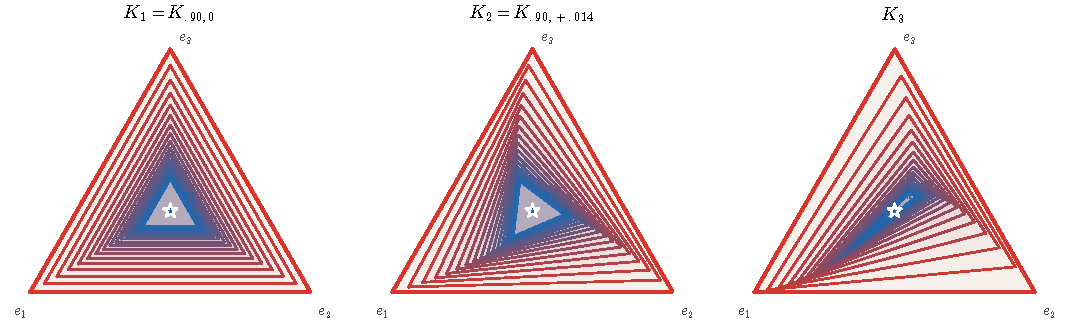
\includegraphics[width=.98\linewidth]{figures/sinkhorn-birkhoff-simplex-contraction--simplex-contraction.pdf}
\caption{\emph{Positive Markov kernels contract the three-state simplex and can simultaneously rotate its image.} Each colored polygon is $\K_i^\ell\simplex_3$: color progresses from red at $\ell=0$ to blue at $\ell=15$, and the star is the common stationary vector $\pi_i=\ones_3/3$. The isotropic kernel $\K_1$ preserves edge directions, $\K_2$ rotates an essentially homothetic triangle, and the non-normal kernel $\K_3$ both turns and strongly elongates the image because its two tangent modes contract at unequal rates. The red boundary contains zero coordinates and is only a geometric reference: positivity sends the first image into the simplex interior, where Hilbert contraction applies.}
\label{fig:sinkhorn-birkhoff-simplex-contraction}
\index{Birkhoff!contraction theorem}% strictindex
\index{Hilbert!projective metric}% strictindex
\end{figure}

The same theorem holds for positive linear maps between proper cones. Order-preserving homogeneous nonlinear maps admit related projective nonexpansiveness and contraction results, but a generic affine map is not covered because projective homogeneity is essential.
\index{positive!linear map}% strictindex

\paragraph{Sinkhorn contraction.}

Each Sinkhorn half-step composes multiplication by a positive kernel, which contracts Hilbert's metric by Theorem~\ref{thm-birkhoff}, with entrywise multiplication and inversion, which are projective isometries. A complete row--column cycle therefore contracts by the square of the kernel factor. The following result, due to Franklin and Lorenz~\cite{franklin1989scaling}, makes this argument precise.
\index{linear!convergence}% strictindex
\index{Sinkhorn!algorithm}% strictindex

\begin{thm}[Projective linear convergence of Sinkhorn]\label{thm-sinkhorn-hilbert-linear}
	Starting from $\vD^{(0)}>0$, use the scaling iterates of~\eqref{eq-sinkhorn} and the associated primal half-step iterates already defined in~\eqref{eq-kl-sinkh-proj}. Fix any optimal scaling pair $(\uD^\star,\vD^\star)$.
	Writing $\la=\la(\K)$, one has
	\eql{\label{eq-convlin-sinkh}
		\Hilbert(\vD^{(\ell)},\vD^\star)
		\leq
		\la^{2\ell}\Hilbert(\vD^{(0)},\vD^\star),
		\qquad
		\Hilbert(\uD^{(\ell+1)},\uD^\star)
		\leq
		\la^{2\ell+1}\Hilbert(\vD^{(0)},\vD^\star).
	}
	Thus the scaling rays converge linearly. After fixing any continuous gauge, their representatives converge, and $\P^{(\ell)}\to\P^\star$ entrywise. The following posterior estimates use the marginal that is not yet exact at the corresponding step; the first holds for $\ell\geq1$ and the second for $\ell\geq0$:
	\eql{\label{eq-convsinkh-control}
		\Hilbert(\uD^{(\ell)},\uD^\star)
		\leq
		\frac{\Hilbert(\P^{(\ell)}\ones_m,\a)}{1-\la^2}
		\qandq
		\Hilbert(\vD^{(\ell)},\vD^\star)
		\leq
		\frac{\Hilbert((\P^{(\ell+1/2)})^\top\ones_n,\b)}{1-\la^2}.
	}
	\eqllead{Lastly,}{eq-convlin-sinkh-prim}{
		\norm{\log(\P^{(\ell)})-\log(\P^\star)}_\infty
		\leq
		\Hilbert(\uD^{(\ell)},\uD^\star)
		+
		\Hilbert(\vD^{(\ell)},\vD^\star),
	}
	where $\P^\star$ is the unique solution of~\eqref{eq-regularized-discr}.
\end{thm}

\begin{proof}
	Entrywise multiplication by a fixed positive vector and entrywise inversion are isometries of Hilbert's metric. Therefore the row map $R(\vD)=\a/(\K\vD)$ and the column map $C(\uD)=\b/(\K^\top\uD)$ are both $\la$-Lipschitz by Theorem~\ref{thm-birkhoff}. Their full-cycle compositions $C\circ R$ and $R\circ C$ are $\la^2$-contractions. Since $\vD^\star=C(R(\vD^\star))$ and $\uD^\star=R(C(\uD^\star))$, iteration gives~\eqref{eq-convlin-sinkh}.

	For any contraction $F$ with factor $q<1$ and fixed point $x^\star$, the triangle inequality gives
	\[
		d(x,x^\star)
		\leq
		d(x,Fx)+d(Fx,Fx^\star)
		\leq
		d(x,Fx)+q\,d(x,x^\star),
	\]
	hence $d(x,x^\star)\leq d(x,Fx)/(1-q)$. Apply this with $q=\la^2$ to the two full-cycle maps. The scaling identities
	\(
		\Hilbert(\uD^{(\ell+1)},\uD^{(\ell)})
		=\Hilbert(\a,\P^{(\ell)}\ones_m)
	\)
	and
	\(
		\Hilbert(\vD^{(\ell+1)},\vD^{(\ell)})
		=\Hilbert(\b,(\P^{(\ell+1/2)})^\top\ones_n)
	\)
	then prove~\eqref{eq-convsinkh-control}.

	Finally, write $\xi_i=\log(u_i^{(\ell)}/u_i^\star)$ and $\zeta_j=\log(v_j^{(\ell)}/v_j^\star)$. Then $\log(\P_{i,j}^{(\ell)}/\P_{i,j}^\star)=\xi_i+\zeta_j$ and $\operatorname{osc}(\xi\oplus\zeta)=\operatorname{osc}(\xi)+\operatorname{osc}(\zeta)$.
	Both plans have total mass one, so $\sum_{i,j}\P_{i,j}^\star e^{\xi_i+\zeta_j}=1$. Consequently $\min(\xi\oplus\zeta)\leq0\leq\max(\xi\oplus\zeta)$, and the sup norm of $\xi\oplus\zeta$ is bounded by its oscillation. This proves~\eqref{eq-convlin-sinkh-prim}.
\end{proof}

\paragraph{Nonlinear Sinkhorn images of the simplex.}
The preceding contraction can be visualized simultaneously for every possible scaling ray, rather than along a single initialization. Using the row and column maps from the proof, define the full-cycle map on the left scaling by
\index{Sinkhorn!full-cycle map}% strictindex
\[
	F_{\uD}(\uD)
	\eqdef
	R(C(\uD))
	=
	\a\oslash\left[\K\left(\b\oslash(\K^\top\uD)\right)\right].
\]
It is positively homogeneous, $F_{\uD}(s\uD)=sF_{\uD}(\uD)$ for $s>0$, and therefore induces the projective self-map
\[
	\widehat F_{\uD}(p)
	\eqdef
	\frac{F_{\uD}(p)}{\dotp{F_{\uD}(p)}{\ones_3}},
	\qquad p\in\simplex_3.
\]
Thus $\widehat\uD^{(\ell)}\eqdef\uD^{(\ell)}/\dotp{\uD^{(\ell)}}{\ones_3}$ follows
$\widehat\uD^{(\ell+1)}=\widehat F_{\uD}(\widehat\uD^{(\ell)})$ when $\ell$ indexes complete Sinkhorn cycles. Since $\widehat F_{\uD}$ maps $\simplex_3$ into itself, its set-valued iterates are nested:
\[
	\widehat F_{\uD}^{\,\ell+1}(\simplex_3)
	=
	\widehat F_{\uD}^{\,\ell}\!\left(\widehat F_{\uD}(\simplex_3)\right)
	\subseteq
	\widehat F_{\uD}^{\,\ell}(\simplex_3).
\]
Unlike the linear images in Figure~\ref{fig:sinkhorn-birkhoff-simplex-contraction}, these sets need not be polygons. Theorem~\ref{thm-sinkhorn-hilbert-linear} quantifies their projective shrinkage: since the first image is strictly positive,
\index{Hilbert!diameter}% strictindex
\[
	\operatorname{diam}_{\Hilbert}\!\left(\widehat F_{\uD}^{\,\ell}(\simplex_3)\right)
	\leq
	\la(\K)^{2(\ell-1)}
	\operatorname{diam}_{\Hilbert}\!\left(\widehat F_{\uD}(\simplex_3)\right),
	\qquad \ell\geq1.
\]
Figure~\ref{fig:sinkhorn-projective-scaling-simplex} reuses the three kernels $\K_i$ from Figure~\ref{fig:sinkhorn-birkhoff-simplex-contraction}, with the same uniform Sinkhorn marginals $\a=\b=\ones_3/3$ in every panel. This isolates the passage from the linear action $\K_i^\ell$ to the nonlinear balancing map $\widehat F_{\uD,i}^{\,\ell}$. The symmetric control remains aligned, $\K_2$ turns the curved images, and the unequal tangent rates of $\K_3$ additionally produce a pronounced anisotropic collapse. Here the kernels are doubly stochastic, so the normalized Sinkhorn fixed ray and stationary Markov vector both equal $\ones_3/3$; they need not coincide for general kernels and marginals.

\begin{figure}[H]
\centering
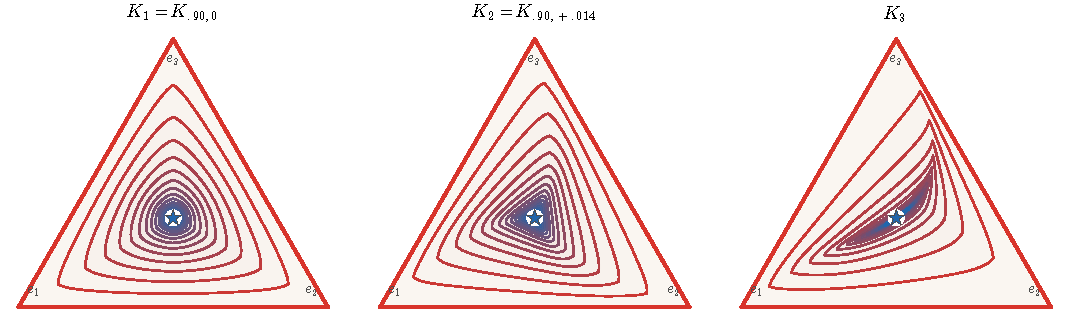
\includegraphics[width=.98\linewidth]{figures/sinkhorn-projective-scaling-simplex--scaling-contraction.pdf}
\caption{\emph{Complete Sinkhorn cycles curve, turn and contract the simplex of normalized left scalings.} Panel $i$ uses the kernel $\K_i$ identified in Figure~\ref{fig:sinkhorn-birkhoff-simplex-contraction} and the common marginals $\a=\b=\ones_3/3$. Color shows the densely sampled boundary of $\widehat F_{\uD,i}^{\,\ell}(\simplex_3)$, progressing from the red triangle at $\ell=0$ to the blue curve at $\ell=15$; the star marks $\widehat\uD_i^\star=\ones_3/3$. Coordinatewise reciprocals curve every image; $\K_2$ adds a gradual turn, whereas the non-normal $\K_3$ combines turning with a much stronger collapse across one tangent direction. Since these kernels are invertible, the projective maps are injective and the sampled curves are the actual boundaries of the nested images. The outer boundary contains zeros; the Hilbert estimate starts after one positive cycle.}
\label{fig:sinkhorn-projective-scaling-simplex}
\index{Sinkhorn!scaling}% strictindex
\index{Hilbert!projective metric}% strictindex
\end{figure}

\paragraph{Dual-potential form of the contraction.}
\index{dual!potential}% strictindex
\index{Birkhoff!contraction theorem}% strictindex

By~\eqref{eq-entropy-pd}, the KL-normalized potentials satisfy
\(
	\fD^{(\ell)}=\epsilon\log(\uD^{(\ell)}\oslash\a)
\)
and
\(
	\gD^{(\ell)}=\epsilon\log(\vD^{(\ell)}\oslash\b)
\).
The Hilbert contraction can therefore be read directly on potential classes because
\[
	\norm{\fD^{(\ell)}-\fD^\star}_V
	=
	\epsilon\Hilbert(\uD^{(\ell)},\uD^\star),
	\qquad
	\norm{\gD^{(\ell)}-\gD^\star}_V
	=
	\epsilon\Hilbert(\vD^{(\ell)},\vD^\star).
\]
Thus a complete cycle contracts both potential classes at the rate $\la(\K)^2$. Moreover, the temperature factor must be retained when passing from potentials to densities:
\eq{
	\norm{ \log \frac{\d\pi^{(\ell)}}{\d\pi^\star} }_\infty
	=
	\frac1\epsilon
	\norm{ (\fD^{(\ell)}-\fD^\star) \oplus (\gD^{(\ell)}-\gD^\star) }_\infty
	\leq
	\frac{\norm{\fD^{(\ell)}-\fD^\star}_V + \norm{\gD^{(\ell)}-\gD^\star}_V}{\epsilon}.
}
Here the last inequality uses the common mass normalization exactly as in the proof of~\eqref{eq-convlin-sinkh-prim}. For the Gibbs kernel $\K_\epsilon=e^{-\C/\epsilon}$, let $R=\max_{i,j}\C_{i,j}-\min_{i,j}\C_{i,j}$. With $\eta=\eta(\K_\epsilon)$ as in Theorem~\ref{thm-birkhoff},
\index{contraction ratio}% strictindex
\index{Gibbs!kernel}% strictindex
\[
	\la=\frac{\sqrt{\eta}-1}{\sqrt{\eta}+1}
	\leq
	\tanh(R/(2\epsilon))<1.
\]
Indeed, every logarithmic kernel cross-ratio is bounded by $2R/\epsilon$. The posterior estimates~\eqref{eq-convsinkh-control} become
\[
	\norm{\fD^{(\ell)}-\fD^\star}_V
	\leq
	\frac{\epsilon}{1-\la^2}
	\norm{\log((\P^{(\ell)}\ones_m)\oslash\a)}_V,
\]
and
\[
	\norm{\gD^{(\ell)}-\gD^\star}_V
	\leq
	\frac{\epsilon}{1-\la^2}
	\norm{\log(((\P^{(\ell+1/2)})^\top\ones_n)\oslash\b)}_V.
\]
These are genuine posterior bounds because they use the marginal that has not yet been normalized.



The marginal violations $\norm{\P^{(\ell)}\ones_m-\a}_1$ and $\norm{(\P^{(\ell+1/2)})^\top\ones_n-\b}_1$ remain useful practical stopping criteria. At each stage one must monitor the marginal that has not just been normalized; these two residuals vanish only as the iteration approaches a common fixed point.
\index{marginal!constraint}% strictindex
Theorem~\ref{thm-sinkhorn-hilbert-linear} shows global linear convergence in projective geometry, but its worst-case rate becomes exponentially bad as $\epsilon\rightarrow0$: $1-\la(\K_\epsilon)^2$ can be of order $e^{-R/\epsilon}$. In practice, one often observes a much better local linear regime after enough iterations, and sharper continuous analyses can replace this exponential dependence by polynomial rates under additional semiconcavity or log-concavity assumptions~\cite{chizat2024sharper}.
\index{Sinkhorn!algorithm}% strictindex
%
The same Hilbert-metric mechanism extends beyond finite matrices to positive integral operators under suitable compactness and positivity assumptions.
%
An important limitation of this analysis is that it requires a uniformly bounded cost and a kernel bounded away from degeneracy; Gaussian distributions with quadratic cost therefore require a different approach.
\index{quadratic!cost}% strictindex

%%%%%%%%%%%%%%%%%%%%%%%%%%%%%%%%%%%%%%%%%%%%%%%%%%%%%%%%%%%%%%%%%%%%%%%%%%%
\section{Local Convergence Analysis and Acceleration}
\label{sec-sinkhorn-local-acceleration}
\index{Sinkhorn!local convergence}% strictindex
\index{Sinkhorn!acceleration}% strictindex

The projective analysis of Section~\ref{sec-sinkhorn-hilbert} gives an initialization-independent global rate from the kernel alone, but this robust bound can be pessimistic near the solution. Linearization reveals a more precise structure: the dual Hessian, the Jacobian of a complete Sinkhorn cycle and the curvature of the entropic semi-dual are all controlled by the same conditional-expectation operator. This operator gives the sharp local factor and motivates two accelerations: over-relaxing the alternating soft transforms, or optimizing the semi-dual after eliminating one potential.

\paragraph{Conditional operator and maximal correlation.}
\index{conditional!expectation}% strictindex
\index{maximal correlation}% strictindex

The local geometry is intrinsic to the coupling and does not depend on whether it is parameterized by potentials or scalings. Let
\(
	L_0^2(\al)\eqdef\enscond{h\in L^2(\al)}{\int h\d\al=0}
\)
and define \(L_0^2(\be)\) similarly.

\begin{defn}[Conditional coupling operator]\label{def-sinkhorn-conditional-operator}
\index{coupling!conditional operator}% strictindex
	For a coupling $\pi\in\Couplings(\al,\be)$, let
	\(
		\pi(\d x,\d y)=\al(\d x)\pi_x(\d y)
		=\be(\d y)\pi^y(\d x)
	\)
	be its two disintegrations. Define
	\(
		T_\pi:L^2(\be)\to L^2(\al)
	\)
	and
	\(
		T_\pi^*:L^2(\al)\to L^2(\be)
	\)
	by
	\eql{\label{eq-sinkhorn-conditional-operator}
		(T_\pi k)(x)\eqdef\int_\Yy k(y)\d\pi_x(y),
		\qquad
		(T_\pi^*h)(y)\eqdef\int_\Xx h(x)\d\pi^y(x).
	}
	The centered maximal correlation of $\pi$ is
	\eql{\label{eq-sinkhorn-maximal-correlation}
		\sigma(\pi)
		\eqdef
		\sup_{\substack{k\in L_0^2(\be)\\\norm{k}_{L^2(\be)}=1}}
		\norm{T_\pi k}_{L^2(\al)}
		=
		\sup_{\substack{h\in L_0^2(\al),\,k\in L_0^2(\be)\\
		\norm{h}_{L^2(\al)}=\norm{k}_{L^2(\be)}=1}}
		\int h(x)k(y)\d\pi(x,y).
	}
	For the optimal entropic coupling $\pi_\epsilon$ of~\eqref{eq-entropic-generic}, set
	\(
		T_\epsilon\eqdef T_{\pi_\epsilon}
	\)
	and
	\(
		\sigma_\epsilon\eqdef\sigma(\pi_\epsilon).
	\)
\end{defn}

The notation $T_\pi^*$ is literal: the two operators are adjoint for the $L^2(\al)$ and $L^2(\be)$ inner products. Conditional Jensen's inequality gives $\norm{T_\pi}\leq1$, while $T_\pi1=T_\pi^*1=1$, so both operators preserve centered functions and $0\leq\sigma(\pi)\leq1$. In the discrete setting of~\eqref{eq-regularized-discr}, assuming the weights are positive, the optimizer $\P_\epsilon$ gives
\eql{\label{eq-sinkhorn-conditional-operator-discrete}
	T_\epsilon=\diag(\a)^{-1}\P_\epsilon,
	\qquad
	T_\epsilon^*=\diag(\b)^{-1}\P_\epsilon^\top,
}
where adjointness is understood in the $\a$- and $\b$-weighted Euclidean inner products. Thus $\sigma_\epsilon$ is the largest nonconstant singular value of the normalized optimal coupling.
Equivalently, it is the second singular value of
\(
	\diag(\a)^{-1/2}\P_\epsilon\diag(\b)^{-1/2}
\),
whose first singular value is one.

\paragraph{Dual Hessian and exact local rate.}
\index{dual!Hessian}% strictindex
\index{Sinkhorn!Jacobian}% strictindex

Recall that $\Dd_\epsilon$ is the continuous dual objective~\eqref{eq-dual-sinkhorn-objective}, its optimizers $(f_\epsilon,g_\epsilon)$ are unique up to the gauge $(f,g)\mapsto(f+s,g-s)$ by Proposition~\ref{prop-entropic-dual-potentials}, and Sinkhorn alternates the soft transforms~\eqref{eq-continuous-dual-sinkhorn-iteration}. The following proposition identifies the linearization of all these objects without redefining them.

\begin{prop}[Dual Hessian and local Sinkhorn rate]\label{prop-sinkhorn-local-rate}
	Assume the setting of Proposition~\ref{prop-continuous-entropic-duality}, and that differentiation under the Gibbs integrals and the stated $L^2$ Taylor expansions are valid. These requirements are automatic in finite spaces and form the local regularity hypothesis in continuous settings. For bounded directions $(h,k)$ and $(h',k')$,
	\eql{\label{eq-sinkhorn-dual-hessian-form}
		-\epsilon D^2\Dd_\epsilon(f_\epsilon,g_\epsilon)
		[(h,k),(h',k')]
		=
		\int_{\Xx\times\Yy}
		(h(x)+k(y))(h'(x)+k'(y))\d\pi_\epsilon(x,y).
	}
	Hence the Hessian form extends continuously to
	\(L^2(\al)\oplus L^2(\be)\), where the positive dual curvature operator is
	\eql{\label{eq-sinkhorn-dual-hessian-operator}
		-\nabla^2\Dd_\epsilon(f_\epsilon,g_\epsilon)
		=
		\frac1\epsilon
		\begin{pmatrix}
			\Id&T_\epsilon\\
			T_\epsilon^*&\Id
		\end{pmatrix}.
	}
	After quotienting by the gauge direction $(1,-1)$ and using the product-$L^2$ quotient norm, its spectrum is contained in $[(1-\sigma_\epsilon)/\epsilon,2/\epsilon]$.
	Both endpoints belong to the spectrum, although the lower one need not be an eigenvalue.
	In particular, when $\sigma_\epsilon<1$, the spectral condition number of the full dual is \(2/(1-\sigma_\epsilon)\).

	The derivatives of the two soft-transform updates~\eqref{eq-soft-c-cont-f}--\eqref{eq-soft-c-cont-g} at the optimum are
	\eql{\label{eq-sinkhorn-soft-transform-jacobians}
		D[g\mapsto g^{\bar c,\epsilon}](g_\epsilon)=-T_\epsilon,
		\qquad
		D[f\mapsto f^{c,\epsilon}](f_\epsilon)=-T_\epsilon^*.
	}
	Consequently, the Jacobian of a complete cycle
	\(g\mapsto(g^{\bar c,\epsilon})^{c,\epsilon}\)
	is $T_\epsilon^*T_\epsilon$. If the gauges are fixed so that
	\(e^{(\ell)}\eqdef g^{(\ell)}-g_\epsilon\in L_0^2(\be)\), then
	\eql{\label{eq-sinkhorn-local-error}
		e^{(\ell+1)}
		=
		T_\epsilon^*T_\epsilon e^{(\ell)}
		+
		o\!\left(\norm{e^{(\ell)}}_{L^2(\be)}\right),
		\qquad
		\limsup_{\ell\to\infty}
		\frac{\norm{e^{(\ell+1)}}_{L^2(\be)}}
		{\norm{e^{(\ell)}}_{L^2(\be)}}
		\leq\sigma_\epsilon^2.
	}
	If $\sigma_\epsilon^2$ is an isolated eigenvalue and the asymptotic error has a nonzero projection onto its eigenspace, the ratio in~\eqref{eq-sinkhorn-local-error} converges to $\sigma_\epsilon^2$.
\end{prop}

\begin{proof}
	Twice differentiating the exponential term in~\eqref{eq-dual-sinkhorn-objective} gives~\eqref{eq-sinkhorn-dual-hessian-form}; the density law~\eqref{eq-continuous-entropic-density-law} identifies its reference measure with $\pi_\epsilon$. Its two diagonal terms are the $L^2$ inner products of the marginals, and its cross term is represented by $T_\epsilon$, which proves~\eqref{eq-sinkhorn-dual-hessian-operator}.

	Each quotient class has a unique representative orthogonal to the gauge direction, hence of the form
	\(
		(h_0+m,k_0+m)
	\)
	with $h_0\in L_0^2(\al)$ and $k_0\in L_0^2(\be)$. On the centered component, Cauchy--Schwarz and~\eqref{eq-sinkhorn-maximal-correlation} give
	\[
		(1-\sigma_\epsilon)
		\bigl(\norm{h_0}_{L^2(\al)}^2+\norm{k_0}_{L^2(\be)}^2\bigr)
		\leq
		\norm{h_0}_{L^2(\al)}^2+\norm{k_0}_{L^2(\be)}^2
		+2\langle h_0,T_\epsilon k_0\rangle_{L^2(\al)}
		\leq
		(1+\sigma_\epsilon)
		\bigl(\norm{h_0}_{L^2(\al)}^2+\norm{k_0}_{L^2(\be)}^2\bigr).
	\]
	The common-constant direction $(1,1)$ has eigenvalue $2/\epsilon$, whereas $(1,-1)$ is the gauge kernel. Approximate maximizers in~\eqref{eq-sinkhorn-maximal-correlation} show that the lower spectral endpoint is $(1-\sigma_\epsilon)/\epsilon$, while the constant direction gives the upper endpoint $2/\epsilon$. This proves the condition-number formula without requiring a singular-vector basis.

	Differentiating either log-partition formula in Definition~\ref{def-continuous-soft-c-transform} produces minus the corresponding conditional expectation under $\pi_\epsilon$, proving~\eqref{eq-sinkhorn-soft-transform-jacobians}. The chain rule and a Taylor expansion then give~\eqref{eq-sinkhorn-local-error}. Since
	\(\norm{T_\epsilon^*T_\epsilon}_{L_0^2(\be)\to L_0^2(\be)}
	=\sigma_\epsilon^2\),
	the rate follows.
\end{proof}

In finite spaces, this recovers the second-singular-value description of the asymptotic matrix-scaling rate~\cite{knight2008sinkhorn,lehmann2022overrelaxation}.

The same spectral gap has a direct probabilistic interpretation. The law of total variance gives
\eql{\label{eq-sinkhorn-conditional-variance-gap}
	1-\sigma_\epsilon^2
	=
	\inf_{\substack{k\in L_0^2(\be)\\\norm{k}_{L^2(\be)}=1}}
	\int_\Xx
	\operatorname{Var}_{\pi_{\epsilon,x}}\!\bigl(k(Y)\bigr)
	\d\al(x).
}
Thus Sinkhorn slows down when the optimal conditional laws $Y|X=x$ become nearly deterministic. This is exactly what happens as $\epsilon\to0$ in a smooth Monge regime.

The global projective contraction must dominate every infinitesimal contraction at its fixed point. The next proposition makes this expected comparison precise, while also showing why the kernel-only Hilbert estimate can be much more pessimistic than the coupling-dependent local factor.

\begin{prop}[The global Hilbert factor controls the local rate]\label{prop-sinkhorn-hilbert-controls-local}
	In the discrete positive-kernel setting of Theorem~\ref{thm-sinkhorn-hilbert-linear}, let $\la(\K)$ be the Birkhoff contraction factor defined in Theorem~\ref{thm-birkhoff}. Then
	\eql{\label{eq-sinkhorn-hilbert-controls-local}
		\sigma_\epsilon\leq\la(\K)<1,
		\qquad
		\sigma_\epsilon^2\leq\la(\K)^2.
	}
\end{prop}
\begin{proof}
	Let $R(\vD)=\a\oslash(\K\vD)$ and $C(\uD)=\b\oslash(\K^\top\uD)$ be the row and column scaling maps used in the proof of Theorem~\ref{thm-sinkhorn-hilbert-linear}. Entrywise inversion and multiplication by a fixed positive vector are isometries of Hilbert's metric. Theorem~\ref{thm-birkhoff}, applied successively to $\K$ and $\K^\top$, therefore gives the pairwise estimate
	\[
		\Hilbert\bigl(C(R(\vD)),C(R(\widetilde\vD))\bigr)
		\leq
		\la(\K)^2\Hilbert(\vD,\widetilde\vD),
	\]
	where $\la(\K^\top)=\la(\K)$ follows directly from its cross-ratio definition. Under the logarithmic change of variables $g=\epsilon\log\vD$, Hilbert's metric becomes $\epsilon^{-1}\norm{\cdot}_V$ by~\eqref{eq-hilbert-metric}. Hence the complete dual update
	\(
		\mathcal S(g)\eqdef(g^{\bar c,\epsilon})^{c,\epsilon}
	\)
	is $\la(\K)^2$-Lipschitz for the variation norm on the quotient by constants:
	\[
		\norm{\mathcal S(g)-\mathcal S(\widetilde g)}_V
		\leq
		\la(\K)^2\norm{g-\widetilde g}_V.
	\]
	Differentiate this inequality at the fixed point $g_\epsilon$. Proposition~\ref{prop-sinkhorn-local-rate} gives
	\(D\mathcal S(g_\epsilon)=T_\epsilon^*T_\epsilon\), and therefore
	\[
		\norm{T_\epsilon^*T_\epsilon h}_V
		\leq
		\la(\K)^2\norm{h}_V
		\qquad
		\text{for every }h\in L_0^2(\be).
	\]
	In the present finite-dimensional setting, $T_\epsilon^*T_\epsilon$ is positive and self-adjoint for the $\be$-weighted inner product, and its largest eigenvalue on $L_0^2(\be)$ is $\sigma_\epsilon^2$. If $\sigma_\epsilon>0$, take a corresponding eigenvector $h_\star$. It is nonconstant, so $\norm{h_\star}_V>0$, and the preceding bound gives
	\[
		\sigma_\epsilon^2\norm{h_\star}_V
		=
		\norm{T_\epsilon^*T_\epsilon h_\star}_V
		\leq
		\la(\K)^2\norm{h_\star}_V.
	\]
	The conclusion is immediate; the case $\sigma_\epsilon=0$ is trivial.
\end{proof}

The same argument applies when the Gibbs kernel is continuous and strictly positive on compact marginal supports: the corresponding optimal coupling has a density relative to $\al\otimes\be$ that is bounded above and below, the conditional operator is compact, and the continuous Birkhoff--Hopf coefficient bounds $\sigma_\epsilon$ strictly below one.

The proposition makes the relation with the preceding section precise: maximal correlation is the sharp local quantity, whereas Birkhoff contraction supplies an input-level global upper bound. The latter can become exponentially close to one as $\epsilon\to0$. In a smooth nondegenerate Monge regime, the conditional laws have width $O(\sqrt\epsilon)$. If a uniform Laplace expansion turns the conditional-variance form in~\eqref{eq-sinkhorn-conditional-variance-gap} into $\epsilon$ times a coercive weighted Dirichlet form, then
\(
	1-\sigma_\epsilon^2\asymp\epsilon.
\)
This explains why observed local rates can be polynomially better than the universal Hilbert estimate. Related non-asymptotic continuous bounds with polynomial dependence on $\epsilon$ are proved under regularity and log-concavity hypotheses in~\cite{chizat2024sharper}; Proposition~\ref{prop-gaussian-sinkhorn-1d-rate} gives an explicit Gaussian instance of the local calculation.

\paragraph{Blockwise over-relaxation.}
\index{Sinkhorn!over-relaxation}% strictindex
\index{successive over-relaxation}% strictindex

Sinkhorn performs exact maximization in one dual block after the other. A minimal acceleration extrapolates each block toward its soft-transform maximizer~\cite{thibault2021overrelaxed,lehmann2022overrelaxation}: for $\omega>0$,
\eql{\label{eq-sinkhorn-block-overrelaxation}
	f^{(\ell+1)}=(1-\omega)f^{(\ell)}+\omega(g^{(\ell)})^{\bar c,\epsilon},
	\qquad
	g^{(\ell+1)}=(1-\omega)g^{(\ell)}+\omega(f^{(\ell+1)})^{c,\epsilon}.
}
The choice $\omega=1$ is the original iteration~\eqref{eq-continuous-dual-sinkhorn-iteration}; $0<\omega<1$ damps the updates, while $1<\omega<2$ over-relaxes them.

\begin{prop}[Optimal local block relaxation]\label{prop-sinkhorn-optimal-overrelaxation}
	Assume the hypotheses of Proposition~\ref{prop-sinkhorn-local-rate} and $\sigma_\epsilon<1$. For every $0<\omega<2$, the iteration~\eqref{eq-sinkhorn-block-overrelaxation} is locally linearly convergent modulo the additive gauge. Its optimal relaxation parameter and corresponding asymptotic factor are
	\eql{\label{eq-sinkhorn-optimal-overrelaxation}
		\omega_\star
		=
		\frac{2}{1+\sqrt{1-\sigma_\epsilon^2}},
		\qquad
		r_\star
		=
		\omega_\star-1
		=
		\frac{1-\sqrt{1-\sigma_\epsilon^2}}
		{1+\sqrt{1-\sigma_\epsilon^2}}.
	}
	For $\omega=1$, the factor is $\sigma_\epsilon^2$, as in Proposition~\ref{prop-sinkhorn-local-rate}.
\end{prop}

\begin{proof}
	Use~\eqref{eq-sinkhorn-soft-transform-jacobians}. The polar decomposition of $T_\epsilon$ and the spectral theorem for $(T_\epsilon^*T_\epsilon)^{1/2}$ reduce the centered linearized iteration to scalar spectral values $s\in[0,\sigma_\epsilon]$; in finite dimensions these are the usual singular values. On the corresponding two-dimensional mode, one relaxed cycle has matrix
	\[
		\mathsf M_\omega(s)
		=
		\begin{pmatrix}
			1-\omega&-\omega s\\
			-\omega s(1-\omega)&1-\omega+\omega^2s^2
		\end{pmatrix},
	\]
	whose characteristic polynomial is $z^2-(2(1-\omega)+\omega^2s^2)z+(1-\omega)^2$.
	The supremum of the root moduli is reached, or approached, as $s\to\sigma_\epsilon$. The two roots of this limiting mode have equal modulus precisely when
	\(\omega^2\sigma_\epsilon^2=4(\omega-1)\).
	The smaller solution is $\omega_\star$ in~\eqref{eq-sinkhorn-optimal-overrelaxation}; at this value both root moduli equal $\omega_\star-1$. Below this threshold the dominant real root decreases with $\omega$, while above it the conjugate-root modulus $\omega-1$ increases. This proves optimality and local convergence for $0<\omega<2$.
	The nongauge constant mode has factor $(1-\omega)^2$ and never dominates these centered modes.
\end{proof}

Set $\delta_\epsilon=1-\sigma_\epsilon^2$. When $\delta_\epsilon$ is small, the exact expression in~\eqref{eq-sinkhorn-optimal-overrelaxation} gives the complete-cycle factor
\[
	r_\star
	=
	\frac{1-\sqrt{\delta_\epsilon}}{1+\sqrt{\delta_\epsilon}}
	=
	1-2\sqrt{\delta_\epsilon}
	+2\delta_\epsilon
	+O(\delta_\epsilon^{3/2}),
\]
instead of $\sigma_\epsilon^2=1-\delta_\epsilon$ for ordinary Sinkhorn. The coefficient two is specific to measuring one complete two-block cycle. Per half-step, the corresponding factor is
\(
	\sqrt{r_\star}=1-\sqrt{\delta_\epsilon}+O(\delta_\epsilon)
\).
This is a local prescription. In the finite positive-kernel setting, the Hilbert estimate used in Theorem~\ref{thm-sinkhorn-hilbert-linear} yields global convergence of the relaxed iteration for the conservative range~\cite{lehmann2022overrelaxation}
\(
	0<\omega<2/(1+\la(\K))
\);
larger choices require the adaptive safeguards analyzed in~\cite{thibault2021overrelaxed,lehmann2022overrelaxation}.

Figure~\ref{fig:sinkhorn-overrelaxation} compares this local prediction with nonlinear iterations. A common ordinary-Sinkhorn warm start places all five runs in the local regime before their relaxation parameters are changed.

\begin{figure}[H]
\centering
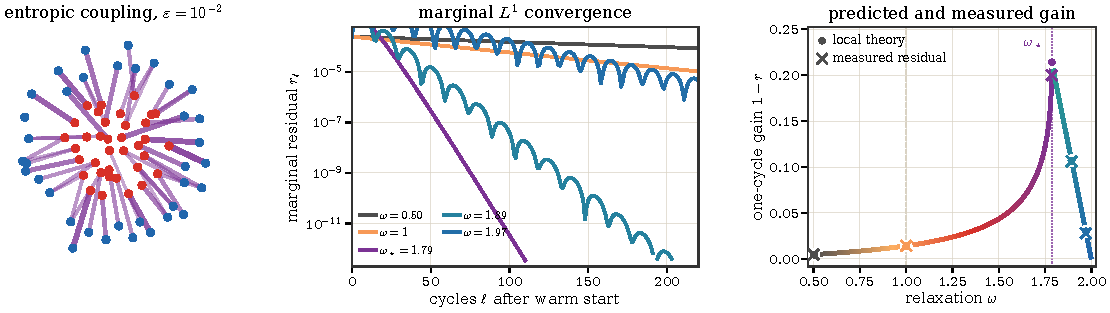
\includegraphics[width=.99\linewidth]{figures/sinkhorn-overrelaxation--overview.pdf}
\caption{\emph{Blockwise over-relaxation accelerates local Sinkhorn convergence.} Left: the entropic coupling at $\epsilon=10^{-2}$; only entries larger than $35\%$ of the maximal mass are drawn, with segment widths proportional to their masses. Middle: after $300$ common ordinary-Sinkhorn warm-up cycles, the residual $r_\ell\eqdef\frac12(\|\P^{(\ell)}\ones-\a\|_1+\|(\P^{(\ell)})^\top\ones-\b\|_1)$ is shown for $\omega\in\{0.5,1,\omega_\star,(\omega_\star+2)/2,1.97\}$; $\omega=1$ is ordinary Sinkhorn, and curves stop at numerical roundoff. Right: the continuous curve is the theoretical one-cycle gain $1-r_{\rm loc}(\omega)$, where $r_{\rm loc}(\omega)$ is the spectral radius of the centered linearization obtained from the maximal correlation $\sigma_\epsilon\simeq0.993$ of the limiting coupling. Filled circles mark this prediction at the five displayed parameters; crosses show the empirical gains $1-\widehat r_{\rm marg}(\omega)$ obtained by fitting $\log r_\ell$ affinely over the final $80$ available iterates above the numerical floor. The palette switches to teal--blue beyond the optimum to distinguish the post-optimal branch of the gain curve. Equation~\eqref{eq-sinkhorn-optimal-overrelaxation} gives $\omega_\star\simeq1.79$.}
\label{fig:sinkhorn-overrelaxation}
\end{figure}

\paragraph{Entropic semi-dual and variable projection.}
\index{semi-dual!entropic}% strictindex
\index{variable projection}% strictindex

The hard semi-dual \(\Ee_0\) in~\eqref{eq-semi-dual} eliminates one potential from the full dual \(\Dd_0\). At positive temperature, the full dual is \(\Dd_\epsilon\) from~\eqref{eq-dual-sinkhorn-objective}, and the soft \(\bar c\)-transform \(g^{\bar c,\epsilon}\) is defined by~\eqref{eq-soft-c-cont-g}. Applying the same partial maximization gives the entropic semi-dual
\eql{\label{eq-entropic-semidual-local}
	\Ee_\epsilon(g)
	\eqdef
	\Dd_\epsilon(g^{\bar c,\epsilon},g)
	=
	\int_\Xx g^{\bar c,\epsilon}\d\al
	+
	\int_\Yy g\d\be.
}
The exponential term disappears in the last equality because the first marginal is normalized by the soft transform. This exact block elimination is an instance of variable projection (VarPro)~\cite{golub1973variableprojection,golub2003variableprojection}. Its general principle is to optimize out one block whenever its conditional optimizer can be computed at acceptable cost. The resulting Schur complement cannot worsen local conditioning, although the size of the improvement is usually unavailable in closed form.

For a potential $g$, let $\pi_g$ be the Gibbs measure obtained from the density law~\eqref{eq-continuous-entropic-density-law} by replacing $(f_\epsilon,g_\epsilon)$ with $(g^{\bar c,\epsilon},g)$. Write
\(
	\pi_g(\d x,\d y)=\al(\d x)\pi_{g,x}(\d y)
\)
and denote its second marginal by $\be_g$. The first marginal is exactly $\al$ by construction.

\begin{rem}[Sinkhorn as an approximate semi-dual gradient ascent]\label{rem-sinkhorn-semidual-gradient}
	Write $r_g\eqdef\d\be_g/\d\be$. Combining the two soft transforms gives
	\eql{\label{eq-sinkhorn-semidual-gradient-comparison}
		r_g
		=
		\exp\!\left(
			\frac{g-(g^{\bar c,\epsilon})^{c,\epsilon}}{\epsilon}
		\right),
		\qquad
		\nabla\Ee_\epsilon(g)=1-r_g,
	}
	where the gradient is taken in $L^2(\be)$. Hence one ordinary Sinkhorn cycle satisfies
	\[
		(g^{\bar c,\epsilon})^{c,\epsilon}-g
		=
		-\epsilon\log r_g
		=
		\epsilon\nabla\Ee_\epsilon(g)
		+o\!\left(\norm{g-g_\epsilon}_{L^2(\be)}\right).
	\]
	Sinkhorn is therefore locally semi-dual gradient ascent with step $\epsilon$, although the nonlinear methods are not globally identical. Quasi-Newton methods instead learn an approximation of $\epsilon(\Id-T_\epsilon^*T_\epsilon)^{-1}$ from successive gradients. This explains the effectiveness of BFGS and L-BFGS on regularized semi-duals~\cite{2016-Cuturi-siims,cuturi2018semidual,nocedal}; stochastic first-order methods exploit the same gradient through sampled marginals~\cite{genevay2016stochastic}. The calculation below quantifies the conditioning improvement produced by eliminating $f$ and thereby gives theoretical support for optimizing the semi-dual directly.
\end{rem}

VarPro was introduced for separable nonlinear least-squares problems. A representative application is training a two-layer network by
\[
	\min_{U,V}\frac12\norm{U\sigma(VX)-Y}_{\rm F}^2,
\]
using the notation $(U,V)$ and activation $\sigma$ of the models studied later in Section~\ref{sec-wasserstein-flows-mlp}. For fixed $V$, optimizing the outer weights $U$ is linear least squares and can be solved by QR, SVD or a linear system at moderate scale; one then optimizes the reduced, generally nonconvex objective in $V$~\cite{kim2008variableprojection}. The present use is structurally different: $(U,V)$ is replaced by the potential pair $(f,g)$, the objective $\Dd_\epsilon(f,g)$ is jointly concave, and the eliminated block has the closed-form maximizer $f=g^{\bar c,\epsilon}$ rather than requiring a linear solve.

\begin{prop}[Semi-dual curvature and conditioning]\label{prop-sinkhorn-semidual-curvature}
	For bounded directions $k,k'$,
	\eql{\label{eq-entropic-semidual-derivatives}
		D\Ee_\epsilon(g)[k]
		=
		\int_\Yy k\d(\be-\be_g),
		\qquad
		D^2\Ee_\epsilon(g)[k,k']
		=
		-\frac1\epsilon
		\int_\Xx
		\operatorname{Cov}_{\pi_{g,x}}\!\bigl(k(Y),k'(Y)\bigr)
		\d\al(x).
	}
	At $g=g_\epsilon$, its positive curvature on $L_0^2(\be)$ is
	\eql{\label{eq-entropic-semidual-hessian}
		-\nabla^2\Ee_\epsilon(g_\epsilon)
		=
		\frac1\epsilon(\Id-T_\epsilon^*T_\epsilon),
		\qquad
		\frac{1-\sigma_\epsilon^2}{\epsilon}\Id
		\preceq
		-\nabla^2\Ee_\epsilon(g_\epsilon)
		\preceq
		\frac1\epsilon\Id.
	}
	Hence its spectral condition number is at most
	\(
		1/(1-\sigma_\epsilon^2)
	\).
\end{prop}

\begin{proof}
	The envelope theorem gives the first derivative in~\eqref{eq-entropic-semidual-derivatives}. Differentiating the normalized conditional Gibbs law gives the covariance formula. At the optimum, total covariance yields
	\[
		\int_\Xx
		\operatorname{Cov}_{\pi_{\epsilon,x}}(k(Y),k'(Y))
		\d\al(x)
		=
		\int_\Yy kk'\d\be
		-
		\int_\Xx(T_\epsilon k)(T_\epsilon k')\d\al,
	\]
	which is~\eqref{eq-entropic-semidual-hessian}. Equivalently, this operator is the Schur complement of the first identity block in~\eqref{eq-sinkhorn-dual-hessian-operator}. Its spectrum on centered functions lies in
	\(
		[(1-\sigma_\epsilon^2)/\epsilon,1/\epsilon]
	\).
\end{proof}

Variable projection cannot worsen local spectral conditioning~\cite{golub1973variableprojection,golub2003variableprojection}: its Hessian is the Schur complement obtained after minimizing the full quadratic form over the eliminated block. In a generic VarPro problem this statement is only qualitative, because the spectra of the full and reduced Hessians depend on several unrelated blocks. Here both diagonal blocks in~\eqref{eq-sinkhorn-dual-hessian-operator} are identities, while the off-diagonal blocks are $T_\epsilon$ and $T_\epsilon^*$. Both condition numbers are therefore controlled by the single number $\sigma_\epsilon$: Proposition~\ref{prop-sinkhorn-local-rate} gives $2/(1-\sigma_\epsilon)$ for the full dual, whereas the semi-dual bound is $1/(1-\sigma_\epsilon^2)$. Thus eliminating $f$ improves the bound by the explicit factor $2(1+\sigma_\epsilon)$.

%%%%%%%%%%%%%%%%%%%%%%%%%%%%%%%%%%%%%%%%%%%%%%%%%%%%%%%%%%%%%%%%%%%%%%%%%%%
\section{Entropic Optimal Transport between Gaussians}
\index{Gaussian!Sinkhorn}% strictindex
\label{sec-gaussian-sinkhorn}

Gaussian marginals provide an explicit finite-dimensional model of Sinkhorn's behavior. The soft $c$-transform preserves quadratic potentials, the optimal entropic coupling is Gaussian, and the value can be written with matrix square roots~\cite{janati2020gaussian}. This is the entropic counterpart of the Gaussian $\Wass_2$ formula in Proposition~\ref{prop-gaussian-w2-bures}.
\index{matrix!square root}% strictindex
\index{soft!c-transform}% strictindex
\index{quadratic!potential}% strictindex
\index{Gaussian!marginals}% strictindex

Gaussian log densities are quadratic, and integrating the exponential of a quadratic against a Gaussian produces another exponential quadratic. This elementary closure turns every Sinkhorn dual iterate into a finite-dimensional matrix recursion.

\begin{prop}[Quadratic closure of Sinkhorn iterates]\label{prop-gaussian-sinkhorn-closure}
\index{quadratic!closure}% strictindex
\index{Sinkhorn!iteration}% strictindex
	Let $\be=\Gaussian(\mean_\be,\cov_\be)$ on $\RR^d$ and take $c(x,y)=\norm{x-y}^2$. If $g(y)$ is a quadratic polynomial such that the Gaussian integral below is finite, then the soft transform
\index{soft!transform}% strictindex
	\[
		f(x)
		=
		-\epsilon\log
		\int
		\exp\!\left(\frac{g(y)-\norm{x-y}^2}{\epsilon}\right)
		\d\be(y)
	\]
	is a quadratic polynomial in $x$.
\end{prop}

\begin{proof}
	The exponent is the sum of a quadratic polynomial in $y$ and the logarithm of the Gaussian density of $\be$. Completing the square in $y$ evaluates the integral as a positive constant times the exponential of a quadratic polynomial in $x$. Taking $-\epsilon\log$ therefore gives a quadratic polynomial.
\end{proof}

Closure of the iterates suggests, but does not by itself prove, that the optimal coupling is Gaussian. Entropy maximization at fixed covariance supplies the missing variational argument and yields the following closed form.

\begin{prop}[Balanced entropic OT between Gaussians]\label{prop-gaussian-sinkhorn-closed-form}
\index{entropic!OT}% strictindex
\index{Gaussian!Sinkhorn}% strictindex
	Let $\al=\Gaussian(\mean_\al,\cov_\al)$ and $\be=\Gaussian(\mean_\be,\cov_\be)$ have positive-definite covariances, and let $\cov_\al^{1/2}\cov_\be^{1/2}=U\diag(\sigma_i)V^\top$ be a singular-value decomposition. For the balanced entropic problem~\eqref{eq-entropic-generic} with $c(x,y)=\norm{x-y}^2$,
	the optimizer is Gaussian with cross-covariance
	\[
		K_\epsilon
		=
		\cov_\al^{1/2}
		U\diag(s_i)V^\top
		\cov_\be^{1/2},
		\qquad
		s_i
		=
		\frac{\sqrt{\epsilon^2+16\sigma_i^2}-\epsilon}{4\sigma_i}.
	\]
	The optimal value is
	\[
		\norm{\mean_\al-\mean_\be}^2
		+
		\tr(\cov_\al)+\tr(\cov_\be)
		+
		\sum_i
		\left(
			-2\sigma_i s_i
			-\frac{\epsilon}{2}\log(1-s_i^2)
		\right).
	\]
	As $\epsilon\downarrow0$, $s_i\to1$ and the full covariance contribution, including the two trace terms, converges to $\Bb(\cov_\al,\cov_\be)^2$.
\end{prop}

\begin{proof}
	Let $(X,Y)$ be any coupling with finite second moments and cross-covariance
	\(K=\EE\big[(X-\mean_\al)(Y-\mean_\be)^\top\big]\).
	Replacing $(X,Y)$ by the Gaussian vector with the same mean and covariance leaves the quadratic cost unchanged. Since the marginals are fixed,
\index{quadratic!cost}% strictindex
	\[
		\KL(\pi|\al\otimes\be)
		=
		-h(X,Y)+h(\al)+h(\be),
	\]
	where $h$ denotes differential entropy when it is finite. Among laws with a fixed covariance, the Gaussian maximizes entropy; if the entropy is not finite, the relative entropy is already $+\infty$. Thus the Gaussian replacement cannot increase the objective, and it is enough to optimize over Gaussian couplings.
\index{relative!entropy}% strictindex

	Any such coupling has covariance
	\[
		\begin{pmatrix}
			\cov_\al & K\\
			K^\top & \cov_\be
		\end{pmatrix}.
	\]
	Write $K=\cov_\al^{1/2}S\cov_\be^{1/2}$. The block covariance constraint is equivalent to the singular values of $S$ being at most one, and finite entropy forces them to be strictly smaller than one. The cost depends on $K$ through
	\[
		\norm{\mean_\al-\mean_\be}^2+\tr(\cov_\al)+\tr(\cov_\be)-2\tr(K),
	\]
	while $\KL(\pi|\al\otimes\be)=-\frac12\log\det(\Id-SS^\top)$.
	By von Neumann's trace inequality, the minimizer aligns $S$ with the singular vectors of $\cov_\al^{1/2}\cov_\be^{1/2}$, so $S=U\diag(s_i)V^\top$. The problem separates into scalar minimizations
	\[
		\min_{0\leq s<1}
		-2\sigma_i s-\frac{\epsilon}{2}\log(1-s^2).
	\]
	The first-order condition is $2\sigma_i=\epsilon s/(1-s^2)$, whose positive solution is the displayed $s_i$. Substitution gives the value formula. Since $s_i\to1$ and $\epsilon\log(1-s_i^2)\to0$ as $\epsilon\downarrow0$, the spectral sum converges to $-2\sum_i\sigma_i$. The identity $\sum_i\sigma_i=\tr((\cov_\al^{1/2}\cov_\be\cov_\al^{1/2})^{1/2})$ then gives the Bures--Wasserstein covariance contribution.
\index{Bures!Wasserstein geometry}% strictindex
\end{proof}

Debiasing the preceding value cancels the marginal trace terms and leaves a smooth spectral deformation of the Bures covariance term.

\begin{cor}[Gaussian Sinkhorn divergence and smoothed Bures term]\label{cor-gaussian-sinkhorn-divergence}
\index{Bures!smoothed term}% strictindex
\index{Sinkhorn!divergence}% strictindex
\index{Gaussian!Sinkhorn divergence}% strictindex
\index{Gaussian!Sinkhorn}% strictindex
	Let $\al=\Gaussian(\mean_\al,\cov_\al)$ and $\be=\Gaussian(\mean_\be,\cov_\be)$ have positive-definite covariances. For $r>0$, define
	\[
		\tau_\epsilon(r)
		\eqdef
		\frac{\sqrt{\epsilon^2+16r^2}-\epsilon}{4r},
		\qquad
		\psi_\epsilon(r)
		\eqdef
		-2r\,\tau_\epsilon(r)
		-\frac{\epsilon}{2}\log\bigl(1-\tau_\epsilon(r)^2\bigr).
	\]
	If $\sigma_i(\Sigma,\Lambda)$ denotes the singular values of $\Sigma^{1/2}\Lambda^{1/2}$ and $\lambda_i(\Sigma)$ the eigenvalues of $\Sigma$, then the debiased Sinkhorn divergence~\eqref{eq-sinkhorn-divergence} is
\index{Sinkhorn!divergence}% strictindex
	\[
		\bar\MK_{\norm{\cdot-\cdot}^2}^{\epsilon}(\al,\be)
		=
		\norm{\mean_\al-\mean_\be}^2
		+
		\Bb_\epsilon(\cov_\al,\cov_\be)^2,
	\]
	where the Gaussian covariance contribution is the debiased smoothed Bures term
\index{Gaussian!covariance}% strictindex
\index{Bures!smoothed term}% strictindex
	\[
		\Bb_\epsilon(\Sigma,\Lambda)^2
		\eqdef
		\sum_i \psi_\epsilon\bigl(\sigma_i(\Sigma,\Lambda)\bigr)
		-\frac12\sum_i\psi_\epsilon\bigl(\lambda_i(\Sigma)\bigr)
		-\frac12\sum_i\psi_\epsilon\bigl(\lambda_i(\Lambda)\bigr).
	\]
	Moreover $\Bb_\epsilon(\Sigma,\Lambda)^2\to\Bb(\Sigma,\Lambda)^2$ as $\epsilon\downarrow0$, where $\Bb$ is the Bures--Wasserstein metric of Proposition~\ref{prop-gaussian-w2-bures}.
\index{Bures!Wasserstein geometry}% strictindex
\end{cor}

\begin{proof}
	Proposition~\ref{prop-gaussian-sinkhorn-closed-form} writes the raw entropic value as the squared mean displacement plus trace terms and a spectral sum. With the notation above, the spectral part is exactly $\sum_i\psi_\epsilon(\sigma_i(\cov_\al,\cov_\be))$. Applying the same formula to the self-costs $(\al,\al)$ and $(\be,\be)$ replaces these singular values by the eigenvalues of $\cov_\al$ and $\cov_\be$. In the polarization formula~\eqref{eq-sinkhorn-divergence}, the trace terms cancel because
\index{Sinkhorn!divergence}% strictindex
	$\tr\cov_\al+\tr\cov_\be-\frac12(2\tr\cov_\al)-\frac12(2\tr\cov_\be)=0$, while the polarization of the squared mean terms leaves exactly $\norm{\mean_\al-\mean_\be}^2$. This gives the displayed formula. Since $\tau_\epsilon(r)\to1$ and $\epsilon\log(1-\tau_\epsilon(r)^2)\to0$, one has $\psi_\epsilon(r)\to-2r$. The limit is therefore
	\[
		\tr\Sigma+\tr\Lambda
		-2\sum_i\sigma_i(\Sigma,\Lambda)
		=
		\Bb(\Sigma,\Lambda)^2,
	\]
	which is the Bures formula~\eqref{eq-bures-defn}.
\end{proof}

The scalar centered case permits an exact non-asymptotic analysis along the invariant family of quadratic potentials. The next result follows the quadratic coefficient itself, rather than the full $L^2$ linearization of a general potential.

\begin{prop}[One-dimensional Gaussian Sinkhorn rate]\label{prop-gaussian-sinkhorn-1d-rate}
\index{Gaussian!Sinkhorn}% strictindex
	Consider $\al=\be=\Gaussian(0,1)$ on $\RR$ with $c(x,y)=(x-y)^2$. Initialize $g^{(0)}=0$ and, after $\ell$ complete Sinkhorn cycles, write
	\[
		g^{(\ell)}(y)=q^{(\ell)}y^2+\mathrm{cst}.
	\]
	One soft transform maps a quadratic coefficient $q$ to
\index{dual!potential}% strictindex
\index{soft!transform}% strictindex
	\[
		\mathsf Q_\epsilon(q)
		=
		1-\frac{1}{1-q+\epsilon/2},
		\qquad q<1+\epsilon/2,
	\]
	so that $q^{(\ell+1)}=\mathsf Q_\epsilon(\mathsf Q_\epsilon(q^{(\ell)}))$. Set
	\[
		A_\ell\eqdef 1-q^{(\ell)}+\frac{\epsilon}{2},
		\qquad
		A_\star\eqdef 1-q_\star+\frac{\epsilon}{2}
		=
		\frac{\epsilon+\sqrt{\epsilon^2+16}}{4}.
	\]
	Then $q^{(\ell)}\to q_\star=1+\epsilon/2-A_\star$, and the convergence obeys the exact cross-ratio identity
	\[
		\frac{A_\ell-A_\star}{A_\ell+A_\star^{-1}}
		=
		A_\star^{-4\ell}
		\frac{A_0-A_\star}{A_0+A_\star^{-1}}.
	\]
	In particular,
	\[
		0\leq q_\star-q^{(\ell)}
		\leq
		q_\star
		\left(\frac{4}{\epsilon+\sqrt{\epsilon^2+16}}\right)^{4\ell}.
	\]
\end{prop}

\begin{proof}
	Completing the square in $\int\exp((q y^2-(x-y)^2)/\epsilon)\d\Gaussian(0,1)(y)$ gives $\mathsf Q_\epsilon(q)$. Write $a=\epsilon/2$. Applying this map twice shows that $A_\ell=1-q^{(\ell)}+a$ satisfies
	\[
		A_{\ell+1}=M(A_\ell),
		\qquad
		M(A)\eqdef a+\frac{A}{1+aA}.
	\]
	The fixed points of $M$ solve $A^2-aA-1=0$ and are $A_\star>0$ and $-A_\star^{-1}$. Direct algebra for this M\"obius map gives
	\[
		\frac{M(A)-A_\star}{M(A)+A_\star^{-1}}
		=
		A_\star^{-4}
		\frac{A-A_\star}{A+A_\star^{-1}},
	\]
	which proves the exact identity by iteration. Moreover, $A_0=1+a>A_\star$ and $M$ leaves $[A_\star,A_0]$ invariant. On this interval,
	\[
		0<M'(A)=\frac{1}{(1+aA)^2}
		\leq
		\frac{1}{(1+aA_\star)^2}
		=A_\star^{-4},
	\]
	where $1+aA_\star=A_\star^2$. Hence $0\leq A_\ell-A_\star\leq A_\star^{-4\ell}(A_0-A_\star)$. Since $A_0-A_\star=q_\star$ and $A_\ell-A_\star=q_\star-q^{(\ell)}$, this is the announced bound.
\end{proof}

Since $A_\star^{-4}=1-\epsilon+O(\epsilon^2)$, reducing the relative coefficient error $(q_\star-q^{(\ell)})/q_\star$ below $\delta$ requires only $O(\epsilon^{-1}\log(1/\delta))$ cycles as $\epsilon\downarrow0$. This is far less pessimistic than the global Hilbert estimate of Theorem~\ref{thm-sinkhorn-hilbert-linear}. On the whole Gaussian space the quadratic cost is unbounded, so that estimate has no finite projective diameter; on a bounded truncation with cost oscillation $R$, it gives a full-cycle factor at most $\tanh^2(R/(2\epsilon))$, whose gap from one is asymptotic to $4e^{-R/\epsilon}$. There is no contradiction: the proposition gives a non-asymptotic rate only along the quadratic Sinkhorn orbit, whose regularity is invisible to the universal projective estimate. It is an explicit instance of the sharper polynomial dependence obtained under regularity assumptions by Chizat, Delalande and Va\v{s}kevi\v{c}ius~\cite{chizat2024sharper}.
\index{Brenier!map}% strictindex


%%%%%%%%%%%%%%%%%%%%%%%%%%%%%%%%%%%%%%%%%%%%%%%%%%%%%%%%%%%%%%%%%%%%%%%%%%%

%%%%%%%%%%%%%%%%%%%%%%%%%%%%%%%%%%%%%%%%%%%%%%%%%%%%%%%%%%%%%%%%%%%%%%%%%%%
\section{Continuous \texorpdfstring{$\varepsilon$}{epsilon}-Sinkhorn Flow}\label{sec-continuous-epsilon-sinkhorn}
\index{Sinkhorn!continuous flow}% strictindex
\index{parabolic optimal transport}% strictindex

This section studies a joint small-temperature and many-iteration limit of Sinkhorn directly on a continuous domain. When the temperature is $\epsilon$ and one cycle is assigned the time step $\epsilon$, the iterates observed after $\lfloor t/\epsilon\rfloor$ cycles formally converge to a parabolic Monge--Amp\`ere equation.

\paragraph{Parabolic Monge--Amp\`ere limit.}
\index{Monge-Ampere@Monge--Amp\`ere!parabolic equation}% strictindex

Take the quadratic torus cost $c(x,y)=d_{\TT^d}(x,y)^2/2$. In the zero-temperature limit, the soft transforms concentrate near the map $x\mapsto x+\nabla u(x)$, while the first Laplace correction records its Jacobian determinant. Rescaling the accumulated correction in iteration time leads to the following flow.

\begin{defn}[Continuous \texorpdfstring{$\varepsilon$}{epsilon}-Sinkhorn flow]\label{def-continuous-epsilon-sinkhorn}
\index{Sinkhorn!continuous flow}% strictindex
	Let $\al$ and $\be$ be probability measures on the unit-volume flat torus $\TT^d$ with smooth positive densities $\density{\al}=e^{-F}$ and $\density{\be}=e^{-G}$. A gauge-fixed potential $u_t:\TT^d\to\RR$, with $\int_{\TT^d}u_t\d x=0$, follows the continuous $\epsilon$-Sinkhorn flow if
	\begin{equation}\label{eq-continuous-epsilon-sinkhorn-pde}
		\partial_t u_t(x)
		=
		\log\det\bigl(\Id+\nabla^2u_t(x)\bigr)
		-G\bigl(x+\nabla u_t(x)\bigr)
		+F(x)-\bar r_t,
	\end{equation}
	where $x+\nabla u_t(x)$ is understood modulo $\ZZ^d$, $\Id+\nabla^2u_t\succ0$, and $\bar r_t$ is the unique scalar preserving the mean-zero gauge.
\index{gauge fixing}% strictindex
\index{Sinkhorn!potential}% strictindex
\end{defn}

The stationary equation is exactly the Jacobian equation for optimal transport, which justifies the geometric form of~\eqref{eq-continuous-epsilon-sinkhorn-pde}.

\begin{prop}[Stationary continuous Sinkhorn potentials]\label{prop-continuous-sinkhorn-stationary}
\index{stationary potential}% strictindex
	Assume that a smooth stationary solution of~\eqref{eq-continuous-epsilon-sinkhorn-pde} satisfies $\Id+\nabla^2u\succ0$, and define $T(x)=x+\nabla u(x)$ modulo $\ZZ^d$. Then $T_\sharp\al=\be$. Conversely, any smooth map of this form satisfying $\Id+\nabla^2u\succ0$ and $T_\sharp\al=\be$ solves the stationary equation, up to the additive gauge of $u$.
\end{prop}

\begin{proof}
	At stationarity, the right-hand side before subtracting $\bar r_t$ is a constant $r$, hence
	\[
		e^{-G(T(x))}\det\nabla T(x)=e^{-F(x)}e^r.
	\]
	The positive Hessian condition makes $T$ an orientation-preserving local diffeomorphism of the torus, homotopic to the identity and therefore of degree one. It is thus a diffeomorphism. Integrating the displayed identity and using that both measures have unit mass gives $e^r=1$. The remaining equality is precisely the change-of-variables formula for $T_\sharp(e^{-F}\d x)=e^{-G}\d x$. Reversing the argument proves the converse.
\index{Jacobian equation}% strictindex
\index{change of variables formula}% strictindex
\end{proof}

\paragraph{Rescaled continuous Sinkhorn iterates.}
\index{Sinkhorn!continuous limit}% strictindex
\index{Laplace method}% strictindex

Let $\mathsf S_\epsilon$ denote one complete continuous dual Sinkhorn cycle~\eqref{eq-continuous-dual-sinkhorn-iteration}, written in the sign convention $u=-f$. Using the soft transforms of Definition~\ref{def-continuous-soft-c-transform},
\[
	\mathsf S_\epsilon u
	\eqdef
	-\Big((-u)^{c,\epsilon}\Big)^{\bar c,\epsilon}.
\]
We fix the additive gauge after every cycle by subtracting the spatial mean. Assigning the time step $\epsilon$ to one cycle then gives the following time interpolation.

\begin{prop}[Rescaled continuous Sinkhorn limit]\label{prop-scaled-log-sinkhorn-limit}
	Let $u_\epsilon^{(0)}=u_0$ be smooth and mean zero, generate
	\[
		u_\epsilon^{(\ell+1)}
		=
		\mathsf S_\epsilon u_\epsilon^{(\ell)}
		-
		\int_{\TT^d}\mathsf S_\epsilon u_\epsilon^{(\ell)}\d x,
	\]
	and define $u_\epsilon(t)\eqdef u_\epsilon^{(\lfloor t/\epsilon\rfloor)}$. In particular, for $\epsilon=1/k$, one observes $u_{1/k}^{(\lfloor kt\rfloor)}$ at time $t$. Assume that, as $\epsilon\downarrow0$, these interpolants converge smoothly on compact time intervals to $u_t$, that $\Id+\nabla^2u_t\succ0$, and that the Laplace expansion below is uniform along the sequence. Then $u_t$ solves~\eqref{eq-continuous-epsilon-sinkhorn-pde}.
\end{prop}

\begin{proof}
	The Laplace expansion of the two soft transforms gives the first-order consistency formula
	\[
		\mathsf S_\epsilon u-u
		=
		\epsilon\left[
			\log\det(\Id+\nabla^2u)
			-G(\Id+\nabla u)+F
		\right]
		+O(\epsilon^2),
	\]
	up to an $x$-independent term, which disappears under the gauge normalization. Dividing the normalized increment by $\epsilon$ and passing formally to the smooth limit gives~\eqref{eq-continuous-epsilon-sinkhorn-pde}; the subtracted spatial mean becomes $\bar r_t$.
\end{proof}

Berman proves a stronger convergence result in which this small-temperature, many-iteration limit is combined with a simultaneous discretization of the continuous marginals on increasingly fine grids~\cite{berman2017sinkhorn}.

\paragraph{One-dimensional Gaussian closure.}
\index{Gaussian!closure}% strictindex

In one dimension, the flow reads
\[
	\partial_tu_t(x)
	=
	\log\bigl(1+u_t''(x)\bigr)
	-G\bigl(x+u_t'(x)\bigr)+F(x)-\bar r_t.
\]
Although it was introduced on the torus, the same formal equation applies on $\RR$ for confining Gaussian densities. Let $\al=\Gaussian(m_\al,\sigma_\al^2)$ and $\be=\Gaussian(m_\be,\sigma_\be^2)$. The equation is closed on quadratic potentials: up to the irrelevant additive constant, write
\[
	x+u_t'(x)=q_t+a_t(x-m_\al),
	\qquad a_t>0.
\]
Substituting this ansatz into~\eqref{eq-continuous-epsilon-sinkhorn-pde} and matching the quadratic and linear coefficients gives the closed two-dimensional system
\eql{\label{eq-continuous-sinkhorn-gaussian-1d}
	\dot a_t
	=
	\frac{1}{\sigma_\al^2}-\frac{a_t^2}{\sigma_\be^2},
	\qquad
	\dot q_t
	=
	-\frac{a_t}{\sigma_\be^2}(q_t-m_\be).
}
The equilibrium is $a_\star=\sigma_\be/\sigma_\al$ and $q_\star=m_\be$, so the stationary affine map is exactly the one-dimensional Gaussian Brenier map. No equation for the additive constant is needed because it is removed by the gauge.
Figure~\ref{fig:sinkhorn-continuous-epsilon-flow} shows this evolution from $u_0=0$ for two pairs of smooth marginals with pronounced density variations.

\begin{figure}[ht]
\centering
\setlength{\tabcolsep}{3pt}
\begin{tabular}{@{}cc@{}}
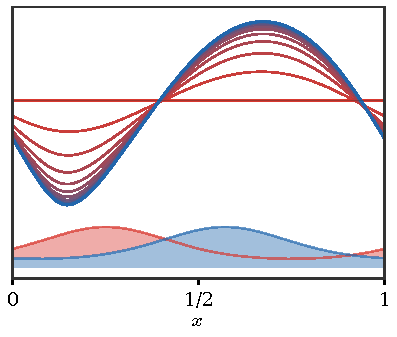
\includegraphics[width=.46\linewidth]{figures/sinkhorn-continuous-epsilon-flow--unimodal.pdf} &
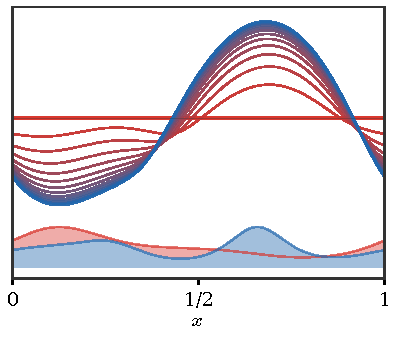
\includegraphics[width=.46\linewidth]{figures/sinkhorn-continuous-epsilon-flow--multimodal.pdf} \\[-.1em]
\small translated high-contrast bump & \small high-contrast multimodal density
\end{tabular}
\caption{\emph{Continuous $\epsilon$-Sinkhorn flow in one dimension.} The curves are snapshots of the gauge-fixed potential $u_t$, initialized at $u_0=0$, under the parabolic Monge--Amp\`ere equation~\eqref{eq-continuous-epsilon-sinkhorn-pde}. Time is encoded from red to blue, while the bottom silhouettes show the source density in red and the target density in blue.}
\index{Monge-Ampere@Monge--Amp\`ere!parabolic equation}% strictindex
\index{Sinkhorn!continuous flow}% strictindex
\label{fig:sinkhorn-continuous-epsilon-flow}
\end{figure}
